% !TeX encoding = UTF-8

%===============================================================================
% Font options are:
%   plain (default), serif (uses Palladio), sans-serif (uses Paratype Sans)
%
% Layout options are:
%   article (default, no chapters), book (for longer texts, offers \chapter)
%   Changing this value between LaTeX runs may require deleting the .aux files
%
% Paragraph options are:
%   noparskip (default, no spacing between paragraphs), parskip (spaced)
%
% Language options are:
%   de (default), en
%   Changing this value between LaTeX runs may require deleting the .aux files
%
\documentclass[serif,article,noparskip,en]{agse-thesis}

% Global parameters, replace with actual values.
\newcommand{\thesisTitle}{Working Memory for Repeated Sentences in Transformer Language Models}
% -> You may use \par (but not \\) to format the title. If you do so, you'll
%    need to manually set the 'pdftitle' attribute below.
\newcommand{\studentName}{Gabriel Arthur Daniel Kressin Palacios}
%===============================================================================

\hypersetup{pdftitle={\thesisTitle}}
\hypersetup{pdfauthor={\studentName}}

\addbibresource{references.bib}
\addbibresource{references_manual.bib}

% Blind texts, for demonstration only, not part of the actual template
\usepackage{lipsum}

\begin{document}

\coverpage[
    student/id=5114015,
    student/mail=gabriel.kressin@fu-berlin.de,
    thesis/type=Bachelor's thesis,            % optional, default: Bachelorarbeit
    thesis/group={},
                                           % optional, default: AGSE
    thesis/advisor={Dr. Kristijan Armeni},           % optional
    thesis/examiner={Prof. Dr. Christopher Honey},
    thesis/examiner/2={Prof. Dr. Eirini Ntoutsi}, % optional
    thesis/date=\today,                    % optional, default: \today
    % title/size=\LARGE,      % set this value to overwrite automatic font size
    abstract/separate,       % toggle this to move the abstract to its own page
]
{ % Your abstract here:
    % !TeX encoding = UTF-8

Language Models (LMs) trained to predict upcoming words in natural language texts are an essential tool in contemporary natural language processing (NLP) research.

In particular, the transformer architecture introduced in 2017 has proven to be especially successful, and transformer LMs have become popular in almost every subdomain of NLP.
Although the architectural features of transformers are determined by human design (e.g. the number of prior words they can access), the internal computations that they learn (e.g. how to use prior context to predict future words) are not well understood.
We theorize that, because the next word prediction objective requires flexibly combining prior context, transformer LMs become functionally organized to possess a high-level mechanism akin to the psychological notion of working memory (WM). In other words, we hypothesize that they specify a limited subset of prior context which has special relevance, and that samples from this subset are  retrieved and manipulated to perform word prediction.


In this thesis, we explore whether the transformer has WM-like capabilities by presenting them with multiple text sequences: a test sequence including the presentation of a sentence in context of the same sentence, and a control sequence including the presentation of the sentence in context of a random sentence.
We propose four concept-models aimed at describing the computational operations of the WM-like capabilities we explore.
Subsequently, we examine five pre-trained transformers -- distilGPT2, GPT2 base, GPT2-medium, GPT2-large and GPT-neo -- across three experiments.
We find that during sentence repetition WM-like mechanisms of transformers are best approximated by a word-semantic-copy-paste mechanism, in which the transformer assigns the highest probabilities to a word and its synonyms, where the word is the exact continuation of the current context in the past.

In conclusion, the thesis introduces a paradigm which allows for numerous experiments to test WM-like capabilities of LMs.
This helps to characterize the algorithmic processes within transformers by drawing on concepts originating in human memory research.

}

\begin{center}\textbf{\small Acknowledgements}\end{center}

First and foremost, I would like to thank Dr. Kristijan Armeni.
His consistent dedicated assistance and lightning-fast responses allowed this project to come to fruition.
The lively discussions we were not only valuable for the thesis, but also provided me with important insights into academia as well.
Moreover, I am very thankful for the continued support in reading and improving almost every section of this thesis.
Thank you for the mentorship, support and understanding.

Furthermore, I wish to express sincere gratitude to Prof. Dr. Christopher Honey.
I am incredibly thankful for Prof. Honey's willingness to supervise this thesis.
His invaluable feedback had an immense impact on the thesis.
Without Prof. Honey's assistance and encouragement it would not have been possible to complete the thesis.
Thank you for the feedback, ideas, comments and the mentorship.

I would like to express my sincere thanks to Fabio Frohberg, Marc Gröling and Friedemann Lohss for their constant support in times of need.
Their willingness to read over the thesis again and again has proven to be a huge alleviation during the final steps of submission.
Thank you for your support and friendship.

Finally, I would like to thank Dr. Tyler Tomita and Savannah Born for reviewing and suggesting synonyms for the wikitext-dataset, and Prof. Dr. Honey and Dr. Armeni for reviewing and suggesting synonyms for the nonce-dataset.

This document is based on the thesis-template created by the working group Software Engineering at Freie Universität Berlin. It can be accessed at \url{https://git.imp.fu-berlin.de/agse/thesis-template/}.


\clearpage

% !TeX encoding = UTF-8
\subsection*{Statement under Oath}

I hereby declare under oath that this paper has not been written by anyone other than myself. All aids used - such as reports, books, websites, or similar - are indicated in the bibliography. Quotations from external works are marked as such. The work has not been submitted to any other examination board in the same or similar form and has not been published before.\\

\thesisDate \\

\studentName

\vspace{20px}
% \includegraphics[width=0.3\textwidth]{misc/signature.png}


\clearpage

\tableofcontents

\cleardoublepage

\pagestyle{fancy}

% Actual content starts here

% !TeX encoding = UTF-8
\section{Introduction}

Language Models (LMs) are computational systems that predict an upcoming word based on previously seen words.
Due to recent improvements to training infrastructure and the introduction of the transformer-architecture \parencite{vaswani_attention_2017}, LMs play an essential role in most subdomains of natural language processing (NLP) \parencite{devlin_bert_2019,brown_language_2020}.

Although the architectural features of transformers are designed carefully by researchers and engineers, the conceptual operations of transformers are not well understood. % explain what is meant with conceptually, (why is it important)
In terms of Marr's three levels \parencite{marr_vision_1982}, the computational level - the computation of an upcoming word based on prior words, and the hardware level - the organization of neurons in layers and the associated implementation are evident.
In contrast, the algorithmic level for transformers is surrounded by mysticism, with some researchers even questioning whether it is possible to find \parencite{lillicrap_what_2019_correct}.
The goal of this thesis is the partial characterization of the algorithmic level in terms of high level algorithmic descriptions.

Hoping to further advance our knowledge of algorithmic operations in the algorithmic level, we theorize that the next word prediction objective during training functionally organizes the inner processes of transformers to develop the capacity to combine and use previous context in a short-term memory buffer, akin to the idea of Working Memory (WM) hypothesized to underpin important aspects of human intelligence.

We propose four algorithmic concept-models aimed at describing how transformers retain and use past context during sentential repetition on a conceptual level: the indiscriminate, plain copy-paste, lexical-syntax copy-paste and lexical-semantic copy-paste concept-model.
To differentiate between the concept-models, we use a paradigm where transformers process sequences in which sentences are repeated twice.
Based on the first presentation of the sentence, we measure how the predictions during the second presentation are affected.
Our goal is to measure how the occurrence of specific features and relationships in the first sentence affects the transformers predictions during the second presentation of the sentence.


\subsection{Working Memory}

In spoken and written language, the meaning of upcoming words is highly dependent on previous context.
Subsequently, well working transformers are able to predict sets of potentially upcoming tokens with high accuracy.
We propose that in the process of learning next-word prediction, transformers develop the capacity to use the information of previous tokens similar to  Working Memory described in psychology.

\paragraph{Working Memory} In psychological and brain sciences it is a common hypothesis that WM is an essential process underpinning human thought and intelligence \parencite{baddeley_working_2003}.
For instance, in the context of language it is essential to maintain and use representations of past words to understand and act in the future.
However, the exact meaning of WM is contentious \parencite{cowan_many_2017}. For the purpose of this work, we refer to WM as:

\begin{definition}
    ``WM refers to a system, or a set of processes, holding mental representations temporarily available for use in thought and action.'' \parencite{oberauer_benchmarks_2018}
\end{definition}

\paragraph{functional Working Memory} We encourage the idea that it may be useful to describe parts of a transformers' inner processes as such a system, which allows for the combination and processing of previous words to predict the new word.
Crucially, we want to highlight the process and abstract away from the underlying architecture. Hence, we introduce the notion of functional WM:

\begin{definition}
    Functional working memory (fWM) refers to a system, or a set of processes operating on sequential data, using past representations to perform a task.
\end{definition}

It is important to differentiate fWM from architectural WM: In the context of LMs, fWM refers to the process of using information from preceding words to predict an upcoming word.
Accordingly, the underlying architecture does not require an explicit mechanism to hold and process representations of previous words:
Although transformers have no architectural WM system, previous context influences their prediction of an upcoming word.
Because a transformers' parameters are initialized randomly, this is a learned capacity: during training transformers learn to take previous tokens into account when predicting upcoming tokens, effectively developing a fWM capability.
Conversely, recurrent neural networks (RNNs) \parencite{elman_finding_1990, mikolov_recurrent_2010} have an explicit architectural mechanism to keep track of previously seen tokens. This architectural bias naturally enforces the model to exhibit a fWM capability
\footnote{Not considering the case in which the model learns to not use the hidden state vector.}.

\paragraph{Long-term Memory vs fWM} Long-term memory refers to the persistent storage of information over a long period of time.
In context of transformers, this refers to the parameters, which are learned during training and then kept unchanged.
On the other hand, we refer to fWM to the effect in which an input is dynamically based on context combined to form an output.
Although the parameters of the transformer are not changed during that process, it is still of major interest to understand how such a dynamical process operates in terms of a high-level description.


\subsection{Testing fWM in Transformers}

We intend to investigate the properties of fWM in transformers.
In ongoing work Armeni et al. investigate the fWM of transformers by introducing a recall paradigm for lists of nouns inspired by the work on benchmarks for models of human WM \parencite{oberauer_benchmarks_2018}.
We expand and adapt the paradigm to sentences.

We present the transformer with two kinds of sequences, a Test-sequence and a Control-sequence.
Both sequences contain a test-sentence placed at the end, and context prior to the test-sentence.
For both sequences, during presentation of the test-sentence, we measure the transformers' surprisal for each word $w$ -- the degree to which the current word was unexpected by the transformer.
This is done by presenting the transformer with the words in the context $w_1 , \dots , w_{n-1}$ and measuring the surprisal for the word $w_n$.
Importantly, the Test-sequence's context stands, because of some feature, in a relationship with the test-sentence.
On the contrary, the Control-sequence's context does not have this feature, and hence not the relationship with the test-sentence.

If the transformers' fWM is able to use the feature of the context in the Test-sequence to predict the words of the test-sentence, a reduction of surprisal will be recorded.
On the other hand, the lack of such a reduction at the test-sentence of the Control-sequence indicates that the context did not contain the information needed to increase the predictability of the test-sentence.
Because we know that the context in the Control-sequence does not stand in relationship with the test-sentence, this demonstrates that the lack of this relationship leads to a lack of the predictability of the test-sentence.
This rules out other sources of surprisal reduction which are not related to context, for example the unigram frequency of words within the test-sentence.
We can then determine the relationships for which the transformer can use context to determine plausible high-level descriptions for the fWM of a transformer.
For details, see section \ref{methods:paradigm}.


\subsection{Concept-models of transformer fWM}

To guide our investigation of fWM in transformers, we propose four concept-models as high-level descriptions of transformer fWM.
Rather than looking at specific mechanisms of how the transformer implements fWM, we focus on a description based upon the transformers' behavior (i.e. output loss) in the context of sentential repetition.
This way, we hope to create a high-level understanding of computational operations in transformers.

On a conceptual level, a proper model of transformer fWM covers two processes:

\paragraph{1. What information is encoded in fWM?} In order to use information from past context for prediction, it has to be determined which information is encoded.
This process is highly context dependent.
For instance, we may imagine a fWM which only during repetition of sentences will start to encode the previous section with most repeated words in current context.
Another fWM might only encode a semantic gist of these words, but not the exact words.

\paragraph{2. Which encoded information is used in fWM and how?} Encoded information can be put to use in different ways.
For example, based on some encoded information, a model may predict similar syntactic structures, whilst another predicts semantically related words.

\paragraph{} The answer to both questions does not need to be limited to one specific process.
On the contrary, as the answers are highly dependent on the context in which the transformer is used, it is very likely that the characterization of transformer fWM by one process alone is insufficient.
Instead, transformer fWM probably has to be characterized in terms of multiple processes working together.

In the following, we describe four concept-models which may be plausible descriptions of transformer fWM operation during sentence repetition.
On the basis of an input sequence of words $w_1, \dots, w_{n-1}$ a transformer predicts a probability distribution over all possible words $w_n$.
The concept-models are formalized by specifying which input words are encoded and how this encoded information affects the probabilities for the words $w_n$.
They mainly differ in the second process.
For the rest of the thesis, we design experiments with the goal of finding an appropriate description of transformer fWM in terms of one or multiple concept-models.

\begin{description}
    \item[M0: Indiscriminate]\hfill \\
        The simplest approach for transformer fWM is the decrease of surprise for any previous word in context. This is akin a  "bag of words" fWM-mechanism - any previously seen word will have a higher probability to be predicted.
        Formally, given input $w_1, \dots, w_{n-1}$, increase the probability of prediction for all $w_n$ with $w_n \in \{w_1, \dots, w_{n-1}\}$.\\

    \item[M1: Plain copy-paste]\hfill \\
        The power of self-attention lies in its context dependency.
        Hence, it is imaginable that the transformer takes the previous words dynamically into account depending on the current context.
        A simple mechanism of such kind is copy-pasting: based on current context, performing verbatim repetition of the previously seen sequence of words.
        Such a plain copy-paste mechanism jumps to the longest matching previous occurrence of the current context and predicts its next word.
        Formally, given the input $w_1, \dots, w_{n-1}$ a plain copy-paste mechanism matches the largest possible current context $w_{n-i}, \dots, w_{n-1}$ word by word with the words of previous context $w_{t-i}, \dots, w_{t-1}$, where $i$ denotes the length of the match, $t$ denotes the position of the matched previous context, and $i < t < w$.
        The plain copy-paste fWM then can encode this previous context $w_{t-i}, \dots, w_{t-1}$ together with its next word $w_t$. Subsequently, the prediction $w_n$ is expected to be the verbatim repetition $w_n = w_{t}$.\\

    \item[M2: Lexical-Syntactic copy-paste]\hfill \\
        We know that transformers can extract certain syntactic features from its input \parencite{rogers_primer_2020}.
        Thus, a more sophisticated method would allow the transformer not only to predict \textit{verbatim} repetition, but instead to consider any other word, as long as it is within the same part-of-speech\footnote{part-of-speech (POS) refers to groups of words with similar grammatical roles. For example, in the sentence \textit{``I like spaceships''} the word \textit{like} is commonly classified in POS-category ``verb''.} (POS) category as the original next word derived from the previous context.
        Formally, we introduce the function $\text{pos}(w)$ which maps words $w$ to their syntactic role.
        Given the same encoding mechanism as M1, the fWM now assigns a word $w_n$ with $\text{pos}(w_n) = \text{pos}(w_{t})$ the highest probability as prediction.\\

    \item[M3: Word-Semantic copy-paste]\hfill \\
        This model is analogous to M2, but instead of allowing arbitrary syntactically appropriate words, it will only predict semantically similar words: synonyms that are contextually appropriate.
        \sloppy Formally, we introduce the function $\text{syn}(w_t | w_{t-i}, \dots, w_{t-1})$ which maps word $w_t$ to its ``semantic category'' based on the given context $w_{t-i}, \dots, w_{t-1}$.
        \sloppy Given the same encoding function as M1 and M2, the word-semantic fWM assigns the highest probabilities to words $w_n$ with $\text{syn}(w_n | w_{n-i}, \dots, w_{n-1}) = \text{syn}(w_t | w_{t-i}, \dots, w_{t-1})$.
        This attribution of probabilities will not happen evenly across all synonyms, but it will be higher for synonyms the transformer deems more fitting.
        In particular, the repeated word $w_t$ is a a great ``synonym'' to itself.

\end{description}

\newpage

% !TeX encoding = UTF-8
\section{Related Work}

\paragraph{Context in LSTMs} Efforts to understand the role of context have preceded the transformer-architecture: One of the most successful architectures was the Long-Short-Term-Memory (LSTM) \parencite{hochreiter_long_1997}. \textcite{linzen_assessing_2016} find that LSTM LMs can capture some grammatical dependencies such as subject-verb-agreement, but do not perform well without strong supervision. \textcite{khandelwal_sharp_2018} measure the effect of context ablations on language modeling accuracy. They truncate, replace and shuffle the context at different positions and find that LSTMs can use up to 200 tokens of context, for which only the order of the first 20 tokens matters.

\paragraph{Context in Transformers} \cite{oconnor_what_2021} introduce the measure of \textit{usable information} in context, to measure the effect of fine grained lexical and structural ablations.
They show that most of the used information by transformers lies in local ordering statistics and content carrying words across a long range.

\paragraph{Interpretability of transformers} There is a considerable amount of publications concerned with understanding transformer function \parencite{rogers_primer_2020}.
However, many studies focus on either diagnosing the extent of knowledge present, or probing for that information within internal transformer structures.
In contrast, this thesis only considers model behavior, thus disregarding any internal theoretical information the model may have, but is not putting to use.

\paragraph{Memory in Neural Networks} An important line of research concerning memory in neural network regards direct architectural integration of memory systems into neural networks.
For example, \cite{nematzadeh_memory_2020} argue for an explicit separation of computation and storage via memory-modules, whilst others analyze, compare and augment transformers and other LMs with different memory architectures  \parencite{yogatama_memory_2022,tay_efficient_2022}.
In this thesis such implementational mechanisms are not the focus, instead we examine context-dependent transformer behavior in terms of high-level descriptions independent of the underlying architecture.

\paragraph{Computational heuristics of transformer function} \cite{mccoy_right_2019} diagnose why statistical models fail in certain cases of natural language inference. They show that the model's function can be described by three heuristics.
In its essence, the heuristics are very similar to our concept-model:
They serve to describe the model's context-based behavior with an approximate high-level description.
The approach used by McCoy et al. make the value of such high-level descriptions evident: based on their heuristics the authors construct a dataset in which the models fail to perform spectacularly.

\paragraph{WM of Transformers} In ongoing work Armeni et al. investigate the WM of transformers and LSTMs.
They introduce a novel paradigm in which surprisal during presentation of repeated noun-lists is measured in order to determine transformer/LSTM recall.
Armeni et al. find that transformers are able to retrieve word identity and position of words in noun lists.
This performance is dependent on learned attention patterns, training corpus size and model depth.
In this thesis, we expand and adapt the paradigm used by Armeni et al. to allow it to work with sentences, furthermore focusing on explanations for transformer behavior.

\paragraph{} In contrast to previous studies we investigate the WM-like capabilities of transformers in order to understand them in terms of high-level computational principles.
This differs vastly from determining how context contributes towards transformer prediction, as it offers -- albeit only for the domain of repeated sentences -- an understandable partial characterization of transformer function.
Moreover, instead of focusing on the information theoretically available within the transformer, we explicitly only take the transformers' output based on the input into account. This shifts the focus to a more practical characterization of actual transformer performance (e.g. it is conceivable that internal word representations encode information the transformer might not be able to use for prediction).

\newpage

% !TeX encoding = UTF-8
\section{Methods}


\subsection{Language Models}
Language Models are computational systems that assign a probability to a word $w_t$ given a sequence of preceding words $w_1, w_2, \dots, w_{t-1}$:
\begin{equation}\label{eq:lm}
    \text{Language Model} = P( w_n | w_1, w_2, \dots, w_{t-1})
\end{equation}
Strictly, LMs operate on tokens and not words. A token is the fundamental unit of text, which can be thought of as word, single character or subword similar to syllables \parencite{sennrich_neural_2016}.
To maintain readability we will use ``word'' instead of ``token''.
All unique words a model can handle are defined as its vocabulary $V$.

A Language Model can also be thought of a system that assigns a probability to a sequence of words $w_1, w_2, \dots, w_t$.
This probability can be factorized into the conditional probability of each word using eq. \ref{eq:lm} and the chain rule:
\begin{equation}
    P(w_1, w_2, \dots, w_t) = \Pi_{i=1}^{t} P( w_i | w_1, w_2, \dots, w_{i-1})
\end{equation}


\subsection{Transformers}
The canonical transformer architecture is characterized by multiple stacks of transformer-blocks, each consisting of a multi-head self-attention layer, feedforward layer, layer normalization and residual connections.
The original transformer introduced in \cite{vaswani_attention_2017} organizes two stacks of transformer-blocks into an encoder and a decoder stack
\footnote{An excellent introduction to transformers can be found in \url{https://nlp.seas.harvard.edu/2018/04/03/attention.html}.}.
Since then, numerous different modifications have been suggested \parencite{tay_efficient_2022}. For instance, \cite{devlin_bert_2019} only use the encoder stack and train their transformer on an adapted version of language modeling. % language modeling is not introduced yet.

The transformers investigated in this thesis use the decoder stack, modeling the conditional distribution of words (eq. \ref{eq:lm}) through successive application of the transformer block to the entire input sequence in parallel  \parencite{radford_improving_2018}:

\begin{equation}\label{eq:transformer}
    \begin{split}
        h_0 &= UW_e + W_p \\
        h_l &= \text{\texttt{transformer\_block}}(h_{l - 1})\quad\forall\; l \in [1,L]\\
        P(w_n | w_1 , \dots , w_{n-1}) &= \texttt{softmax}(h_LW_e^T)
    \end{split}
\end{equation}

where $U = (w_1 , \dots , w_{n-1} )$ is the context vector of words, $L$ is the number of layers, $W_e$ is the word embedding matrix, and $W_p$ is the position embedding matrix.
The transformer block is illustrated in fig \ref{fig:transformer_block}.


\subsection{Language Modeling}
Language modeling (also: causal language modeling) refers to the task of predicting word $w_n$ in context of a preceding sequence of words $w_1, w_2, \dots, w_{n-1}$.
This prediction happens in the form of estimating a probability distribution over $V$.
\begin{equation}
    \text{Probability for $w$ at position $n$ given $w_1, w_2, \dots, w_{n-1}$} = P(w_n | w_1, w_2, \dots, w_{n-1})
\end{equation}
The language model is trained by minimizing the negative log likelihood (NLL)\footnote{Working with the negative log likelihood instead of probabilities has the benefit of numerical stability, as probability values are abysmally small due to large vocabularies in the size of ten-thousands. It is also mathematically valid, because the negative log operation results in a monotonic result that is bigger than 0.} over each word in all sequences $seq$ within the training set $T$:
\begin{equation}
    \text{NLL}(T) = - \frac{1}{|T|} \sum_{\text{seq} \in T} \sum_{w_i \in \text{seq}} \log\left(P(w_i | w_1, w_2, \dots, w_{i-1})\right)
\end{equation}


\subsection{Surprisal}
Formally, the surprisal of a word $w_n$ is defined as the negative log likelihood of the probability that the LM assigns the word $w_n$ at position $n$ given its preceding context $w_1, \dots, w_{n-1}$. It is measured in \textit{bits}:
\begin{equation}
    s(w_n) = - \log_2{P(w_n | w_1, \dots, w_{n-1})}
\end{equation}
In other words, surprisal is used to measure the degree to which a LM ``expected'' the word $w_n$ to occur at position $n$. The higher the surprisal, the less the model has expected to see the word and vice-versa.
In cases when a word is split into multiple sub-words by the byte-pair encoding tokenizer, the surprisal values of the sub-words are summed\footnote{This is valid because the underlying probabilities are not changed: $\log{xy} = \log{x} + \log{y}$}.


\subsection{Paradigm} \label{methods:paradigm}

To test the fWM of a transformer, we present it with a Test-sequence $\text{seq}_T$ and multiple Control-sequences $\text{seq}_{\text{C}} = \left\{ \text{seq}_{\text{C}}^1, \dots, \text{seq}_{\text{C}}^{n_{\text{c}}} \right\}$.
Each Test-sequence is paired with $n_C = 10$ Control-sequences\footnote{We chose $n_C = 10$ because our final measurement stabilizes very quickly, see appendix \ref{app:rs_10_controls}.}, whereby the Test-sequence represents the "Test" and the Control-sequences the "Controls".
Both are jointly constructed.
After construction, we measure the surprisal for each word in the Test-sequence and all Control-sequences:
For every word in a sequence we give all its preceding words as inputs to the transformer and record the surprisal of that word in the output distribution of the transformer.
The surprisal values of Test-sequences are averaged to provide a baseline for the surprisal values in the Test-sequence.
The average from the Test-sequences and the value from the Control-sequence are then finally combined, to obtain a \textit{measure} of repeat surprisal (see \ref{ch:rs}).

\begin{wrapfigure}{L}[0pt]{0pt}
    \centering
    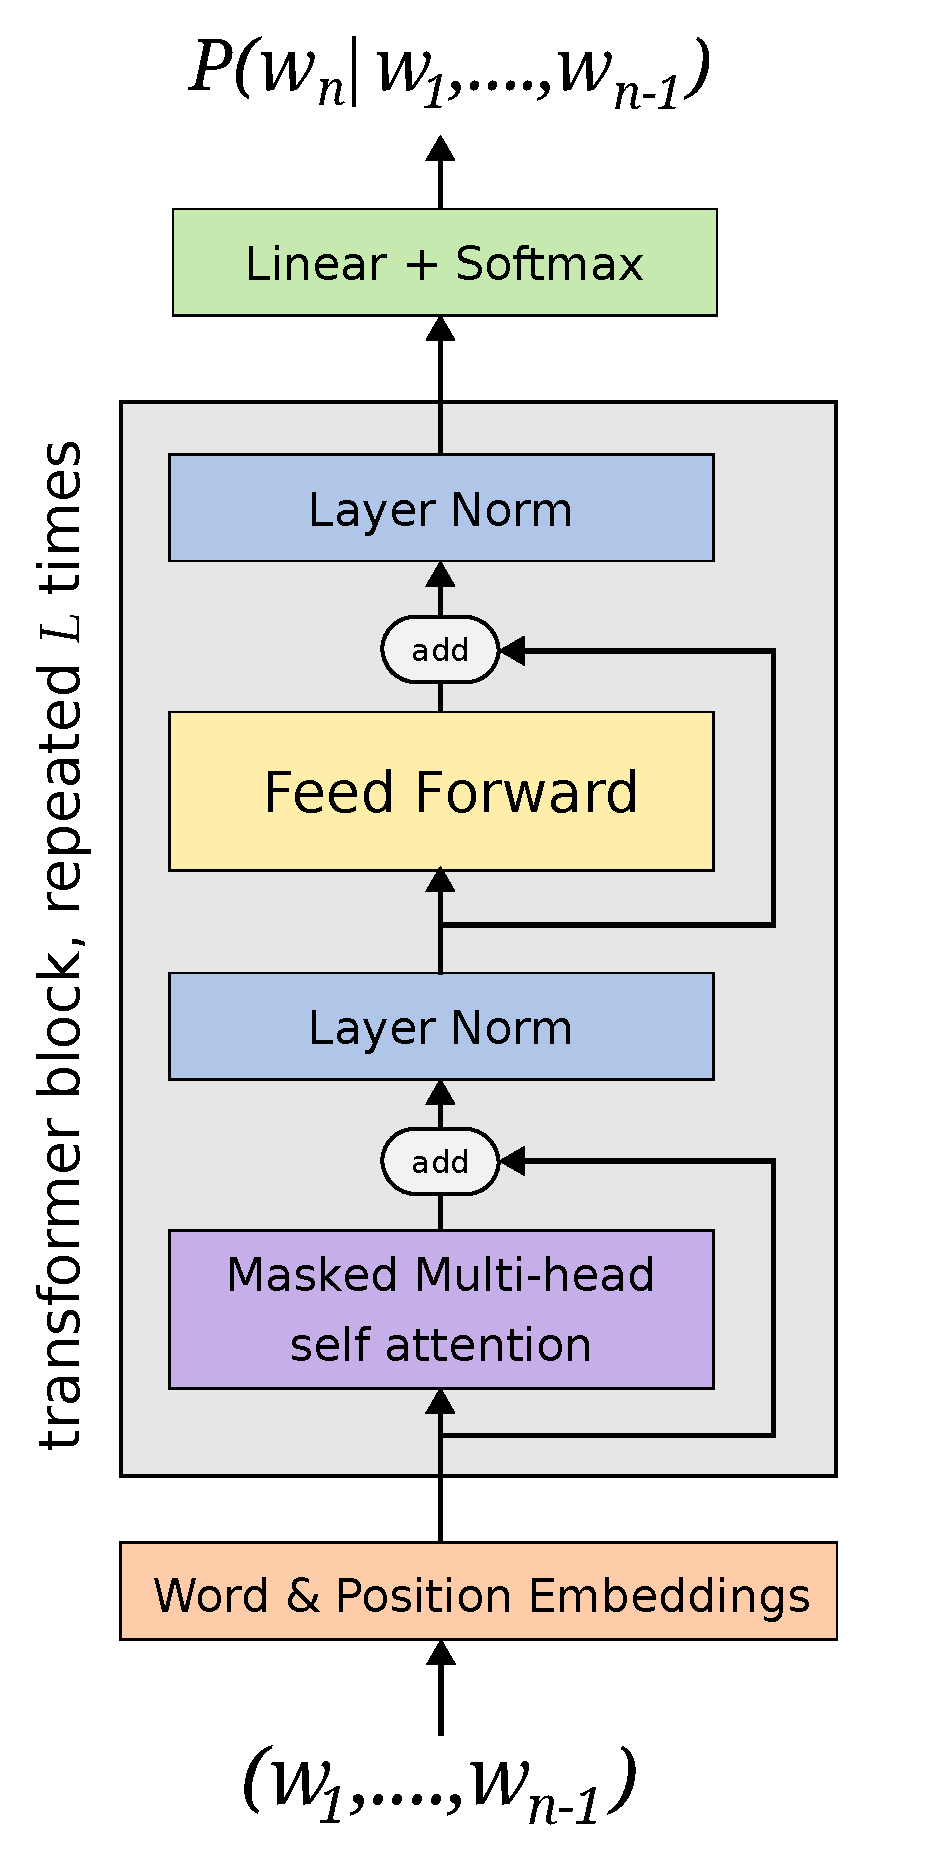
\includegraphics[width=0.4\textwidth]{methods/transformer_block.pdf}
    \caption{Transformer architecture. Input words are embedded and augmented with positional embeddings (orange). The outputs of the embedding layer are fed into the transformer block (grey), which is repeated $L$ times. The last transformer block feeds the outputs into a linear+softmax layer to compute the probability distribution for the next word.}
    \label{fig:transformer_block}
\end{wrapfigure}

The Test-sequence $\text{seq}_T$ and Control-sequences $\text{seq}_{\text{C}}^x$ are constructed from multiple sections:
\begin{center}
    $\text{seq}_{\text{T}}$: \textit{preface}, \textit{encoding-sentence}, \textit{intervention}, \textit{test-sentence}.\\
    $\text{seq}_{\text{C}}^x$: \textit{preface}, \textit{control-sentence}, \textit{intervention}, \textit{test-sentence}.\\
\end{center}
The \textit{preface} is a fixed string that introduces the encoding-sentence (e.g. ``Before the meeting, Mary wrote down the following sentence:'') and is shared by the Test-sequence and the Control-sequence.
In the Test-sequence, the preface is followed by the \textit{encoding-sentence} (e.g. ``the section on current routes adds nothing to the info.'').
The encoding-sentence has a certain relationship with the test-sentence at a later position in the sequence.
In contrast, the \textit{control-sentence} in the Control-sequence is a random sentence that does not have this relationship with the test-sentence (e.g. ``the investigation of chaperones has a long history.'').
At third position follows the \textit{intervention}, a fixed string shared by the Control-sequence and Test-sequence continuing the narrative of the preface and introducing the following section with a short prompt (“After the meeting, Mary took a break. After she got back, she read the sentence again:”).
Finally, the intervention is followed by the \textit{test-sentence} (e.g. “the section on current routes adds nothing to the info.“).

Surprisal reduction on the test-sentence in the Test-sequence would imply that the transformer is able to use the previous context within the Test-sequence to predict the presentation of the test-sentence.
Lack of such surprisal reduction on the test-sentence of the Control-sequence conversely would imply that the transformer cannot use the previous context to predict the presentation of the test-sentence.
As the only difference between the Test-sequence and the Control-sequence are the encoding-sentence and control-sentence, we know that their different relationship to the test-sentence is the source of the surprisal reduction.
This rules out other sources of surprisal reduction which are not related to context, for example the unigram frequency of words within the test-sentence.
Given the appropriate identification of difference in the relationship separating encoding-sentence and control-sentence in respect to the test-sentence, we may now say that the transformer maintained and accessed this relationship in its fWM for next-word-prediction.

The identification of relationships which the fWM of a transformer can use, allows us to characterize the transformers fWM in terms of high-level mechanisms which allow for the use of the feature.
For instance, we may find that the transformers surprisal for the test-sentence is very low when the encoding-sentence is the same as the test-sentence, compared to the surprisal of the test-sentence given a random control-sentence. In such a case, we may denote our feature as "verbatim recall" and describe the fWM of the transformer with a plain copy-paste mechanism.


\subsection{Repeat Surprisal}\label{ch:rs}
In order to quantify the extent to which a LM is able to retrieve specific features from the encoding-sentence (e.g. sentence semantics), we use the notion of \textbf{repeat surprisal}.

We start by taking the surprisal values $\hat{s}$ of the \textit{test-sentence} in the Test-sequence and Control-sequence.
\begin{align}
    \hat{s}\left(\text{seq}_T\right) &:= \left\{\left(w_i, s(w_i)\right) | w_i \in \textit{test-sentence}\;\text{of seq}_T\right\}\\
    \hat{s}\left(\text{seq}_C^x\right) &:= \left\{\left(w_i, s(w_i)\right) | w_i \in \textit{test-sentence}\;\text{of seq}_C^x\right\}
\end{align}
Next, we apply a function $f$ on $\hat{s}$ which yields a scalar.
For instance, $f$ can be the mean, an indexing function returning a specific word or the median:
\begin{equation}\label{eq:f_median}
    f_{\text{median}}\left(\left\{\left(w_1, s(w_1)\right), \dots \right\}\right) := \text{median}\left\{s(w_1), s(w_2), \dots \right\}
\end{equation}
Then, the computed value for a Test-sequence $f\left(\hat{s}\left(\text{seq}_T\right)\right)$ is normalized by the average of the computed values across all the corresponding Control-sequences $f\left(\hat{s}\left(\text{seq}_C^i\right)\right)$.
To yield a percentage, the result is multiplied with 100.
\begin{equation}\label{eq:repeat_surprisal}
    \texttt{repeats surprisal}_f\left(\text{seq}_T, \text{seq}_C\right) := \frac{f\left(\hat{s}\left(\text{seq}_T\right)\right)}{\underset{x}{\text{avg}}\left(f\left(\hat{s}\left(\text{seq}_C^x\right)\right)\right)}\:100
\end{equation}

Here, $f\left(\hat{s}\left(\text{seq}_T\right)\right)$ measures the effect that the encoding-sentence has on the test-sentence.
To make the value interpretable, we divide it by $\underset{i}{\text{avg}}\left(f\left(\hat{s}\left(\text{seq}_C^i\right)\right)\right)$, which measures the average effect any other context (control-sentence) has on the test-sentence.
In other words, $\underset{x}{\text{avg}}\left(f\left(\hat{s}\left(\text{seq}_C^x\right)\right)\right)$ acts as a normalizer for $f\left(\hat{s}\left(\text{seq}_T\right)\right)$.

This method of quantification allows to inspect, in a model agnostic manner, how features of the past context affect the behavior of transformers: by comparing how test-sentence surprisal changes as a function of specific encoding-sentence features, expressed relative to baseline surprisal in control-sentences, we can test what contextual features shape LM's "expectations".
That is, by carefully isolating the target features of the encoding-sentence (e.g. verbatim repetition/identity, semantics, syntax), we can indirectly draw careful conclusions about the transformers fWM capabilities.

The repeat surprisal has the useful quality that it ensures it is in fact a specific feature of the encoding-sentence in respect to the test-sentence which drives the effect on repeat surprisal instead of properties of the vignette (preface, intervention) or test-sentence itself.
For example, if a feature of the vignette (e.g. the intervention's length) or a feature of the test-sentence (e.g. it contains highly probable words) have an impact on surprisal values (and they certainly do), these features will affect \textbf{both} the Test-sequence and the Control-sequences similarly, cancelling out in the division in eq. \ref{eq:repeat_surprisal}.
For this reason, only the \textbf{difference in features} between encoding-sentence and control-sentences in respect to test-sentence is driving the effect.

\begin{figure}
    \centering
    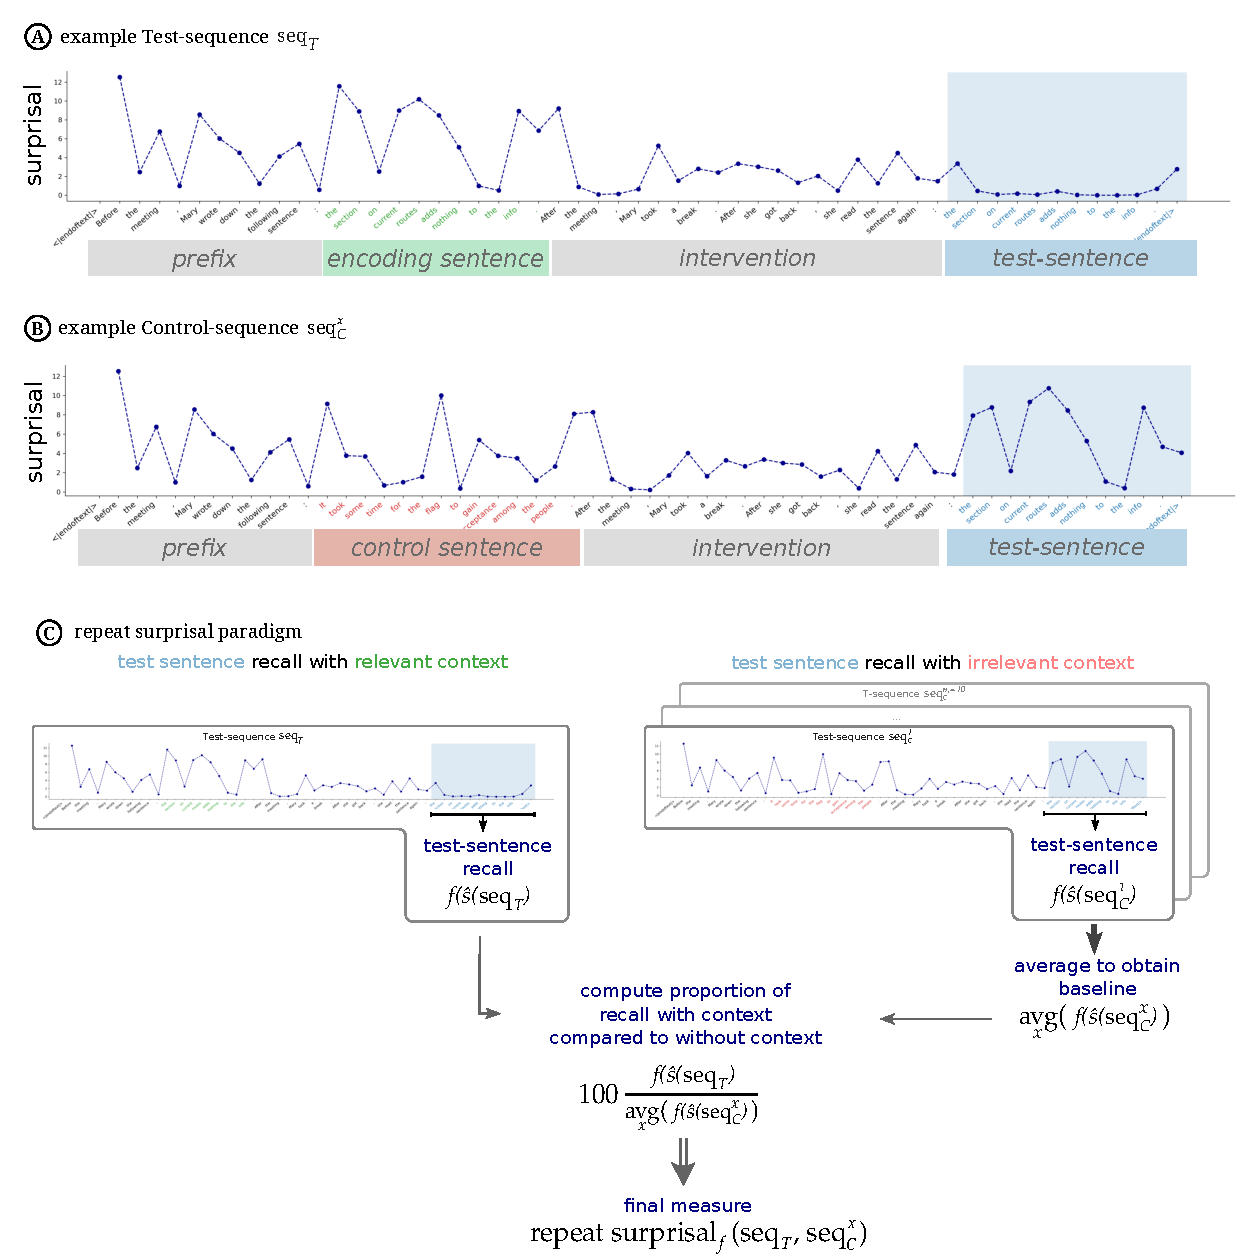
\includegraphics[width=\textwidth]{methods/paradigm.pdf}
    \caption{The paradigm and example surprisal plots. \textbf{A}: Example Test-sequence $\text{seq}_T$: \textit{preface} (grey), \textit{encoding-sentence} (green), \textit{intervention} (grey), \textit{test-sentence} (blue). \textbf{B}: Example Control-sequence $\text{seq}_C^x$ : \textit{preface}, \textit{control-sentence} (red), \textit{intervention}, \textit{test-sentence}. \textbf{C}: Repeat surprisal computation with Test-sequence $\text{seq}_T$ and Control-sequence $\text{seq}_C^x$. From the surprisal values of the test-sentence a single value is computed with $f$. For the Control-sequences these are averaged. The result from the Test-sequence is divided by the averaged result of the Control-sequences and multiplied by 100 to obtain one \textit{measure} of repeat surprisal.}
\end{figure}


\subsection{Repeat Surprisal interpretation}
Given the Test-sequence and Control-sequence, the repeat surprisal has some general implications:

\paragraph{A repeat surprisal percentage close to 0}
indicates that the encoding-sentence provides the LM's WM with context which leads the model to strongly "expect" the test-sentence, whilst the control-sentence does not provide such context.
The encoding-sentence contains some relevant feature to predict the test-sentence, and - importantly - the LM is able to extract and use that feature in its WM.
It is not necessary that the feature aligns with the intuition of a human observer.

\paragraph{A repeat surprisal percentage below 100, but not close to 0}
indicates that the LM is able to extract the relevant information from the encoding-sentence to be less surprised at presentation of the test-sentence, but this information is not definitive enough to make the model strongly expect the test-sentence. This is not necessarily a sign that the model is failing to extract some feature, but instead indicates that the model distributes its expectation over multiple possible test-sentences. Again, the feature the model extracts does not have to align with human intuition.
\paragraph{A repeat surprisal percentage at/around 100}
indicates the LM is not able to extract any relevant information from the given encoding-sentence to predict the test-sentence. In other words, to the LM the encoding-sentence provides as little information as the control sentences. In the case in which a human observer can use some feature from the encoding-sentence in order to be less surprised at presentation of the test-sentence, we can deduce that the model is unable to extract such a feature in at least some cases. The more data points of such nature we collect, the more we can conclude the LM's WM is not capable of operating with such a feature in the encoding-sentence. % a bit more careful here probably. Maybe add "for certain situations"
\paragraph{A repeat surprisal percentage over 100}
indicates the LM is able to extract relevant information from the encoding sentence to \textit{not} expect the test-sentence. In other words, the feature used by the LM's WM encodes something significantly different from what is given in the test-sentence. Again, such an observation may or may not align with human intuition.


\subsection{Sentences used}\label{met:sentences_used}

\paragraph{nonce-sentences}
The first source for the used sentences is the nonce stimulus dataset \cite{wei_frequency_2021} - a dataset containing 300 nouns, 200 verbs and 57 sentence templates.
Each template has one correct noun and verb pair associated with it.
The sentences were revised and filtered, such that in the end we are left with 35 syntactically correct and semantically plausible sentences.
Each sentence has a marked verb and noun. For examples, see \ref{ap:nonce_sentences}.

\paragraph{wikitext sentences}
To introduce a more diverse set of sentences, we used a second set of sentences.
These sentences are sampled from Wikitext103 \parencite{merity_pointer_2016}.
Verbs and nouns were pre-marked with \parencite{van_nguyen_trankit_2021} and then revised and filtered, such that we supplement our pool of sentences by another 25 sentences.

\subsection{Transformers used}

The models are chosen to include varying model sizes and cover different levels of performance.
An overview is provided in table \ref{Tab:models_used}. We used the Hugging Face library \parencite{wolf_transformers_2020}\footnote{\url{https://huggingface.co/}} to access the transformers.\\
\\
\textbf{distilGPT2} is a small version of the same architecture as GPT2. It was trained with GPT2 as supervisor on 38GB of the OpenWebTextCorpus \parencite{gokaslan_openwebtext_2019}. \\
\textbf{GPT2} is a model published by OpenAI mainly based on GPT \parencite{radford_language_2019}.
It uses only the decoder part of the original Transformer.
GPT2 is trained with a LM objective on 40GB of data mined from the internet.
In addition to its base version we used \textbf{GPT2-medium} and \textbf{GPT2-large} as well.
Both differ in their parameter size and amount of transformer block layers to GPT2.\\
\textbf{GPT-neo} is the open source implementation of GPT3.
It is similar in architecture to GPT2, but vastly bigger in size.
GPT-neo is trained on ``The Pile'' \parencite{gao_pile_2020}, a massive dataset of 800GB extracted from the internet with an emphasis on bias and fairness.\\

\begin{table} \centering
    \begin{threeparttable}
        \begin{tabular}{l c c c c }
            \hline
            \thead{Transformer} & \thead{Training\\corpus size}&\thead{Parameters \\ \#} & \thead{WikiText103 \\ (PPL)} \\
            \hline\hline
             distilGPT2     & 38GB & 82M & -\tnote{++}\\
             GPT2-base     & 40GB & 117M & 37.50\tnote{+}\\
             GPT2-medium   & 40GB & 345M & 26.37\tnote{+}\\
             GPT2-large    & 40GB & 762M & 22.05\tnote{+}\\
             GPT-neo & 800GB & 1.3B & 13.10\tnote{*}\\
             \hline
        \end{tabular}
        \begin{tablenotes}\footnotesize
            \item[+] from \textcite{radford_language_2019}
            \item[*] from \url{https://github.com/EleutherAI/gpt-neo/}
            \item[++] ppl without fine-tuning not reported by model creators
        \end{tablenotes}
        \caption{The different pretrained transformers tested in our experiments. They mainly differ in their number of parameters and training corpus size. All transformers are based on the decoder-only architecture \parencite{radford_improving_2018}.} \label{Tab:models_used}
    \end{threeparttable}
\end{table}\textbf{}

\subsection{Implementation}

The entire code to replicate the results and the raw data for each experiment are available at the following github repository: \url{https://github.com/GabrielKP/transformer_wm}.

The implementation is based on an ongoing private codebase from Kristijan Armeni. We realized the project in python, using pytorch \parencite{paszke_pytorch_2019_correct} as neural network framework and the huggingface library \parencite{wolf_transformers_2020} to access transformers. We use numpy \parencite{harris_array_2020_correct} for vectorized operations and pandas \parencite{reback_the_2020_correct} for data management. Plots are created with seaborn \parencite{waskom_seaborn_2021_correct} and matplotlib \parencite{hunter_matplotlib_2007_correct}.

\newpage

\section{Experiments}

\subsection{Repeat Experiment: Do transformers recall sentences?} \label{ex:1_repeat}

Although it is known from Armeni et al. that transformers are able to do verbatim recall for lists of nouns, it is not clear that this effect translates to sentences.
In contrast with lists of arbitrary nouns, sentences are not mere enumerations of words. Instead, words in sentences follow additional structure and constraints which are available to transformers during learning and processing: sentence semantics and syntax.
For example, a transformer may have learned during training that a ``car'' frequently co-occurs with the phrase ``four wheeled vehicle'' and subsequently will assign a higher probability to the token ``car'' when probed for recall of a sentence which includes the phrase ``four wheeled vehicle''.
Second, recall of a specific sentence can stand in competition with similar syntactic structures within the training data.
Therefore, the aim of the first experiment is to determine whether the transformer is able to perform verbatim recall for sentences.

\subsubsection{Experimental Setup}
In this experiment, the encoding-sentence and test-sentence are the same sentence, whilst the control-sentences are sentences randomly sampled from the dataset.
Thus, the feature differing between the encoding-sentence and the control-sentence is verbatim repetition.
If the model is able to recall features of the encoding-sentence, then the repeat surprisal should be significantly less than $100$ percent.

Repeat surprisal is computed by taking the median surprisal value of the test-sentence\footnote{The choice of the median is due to it being less susceptible to outliers than the mean. Effectively, using the mean over the median empirically made no significant difference in any of the experiments.}.
\sloppy Formally, we use $f_\text{median}$ introduced in eq. \ref{eq:f_median} and can compute the $\texttt{repeat surprisal}_{f_\text{median}}$ with eq. \ref{eq:repeat_surprisal}.

\subsubsection{Results} \label{ex:1_repeat_results}

With an average repeat suprisal of $1.65\%$ and a median of $0.82\%$ the repeat suprisal measures for the repeat experiment floor close to $0\%$ (Figure \ref{fig:repeat_gpt2}). These results generalize across the other transformers (Figure \ref{fig:repeat_all}). Moreover, almost all repeat surprisal measures except for a few outliers fall below $5\%$.

\begin{wrapfigure}{R}[0pt]{0pt}
    \centering
    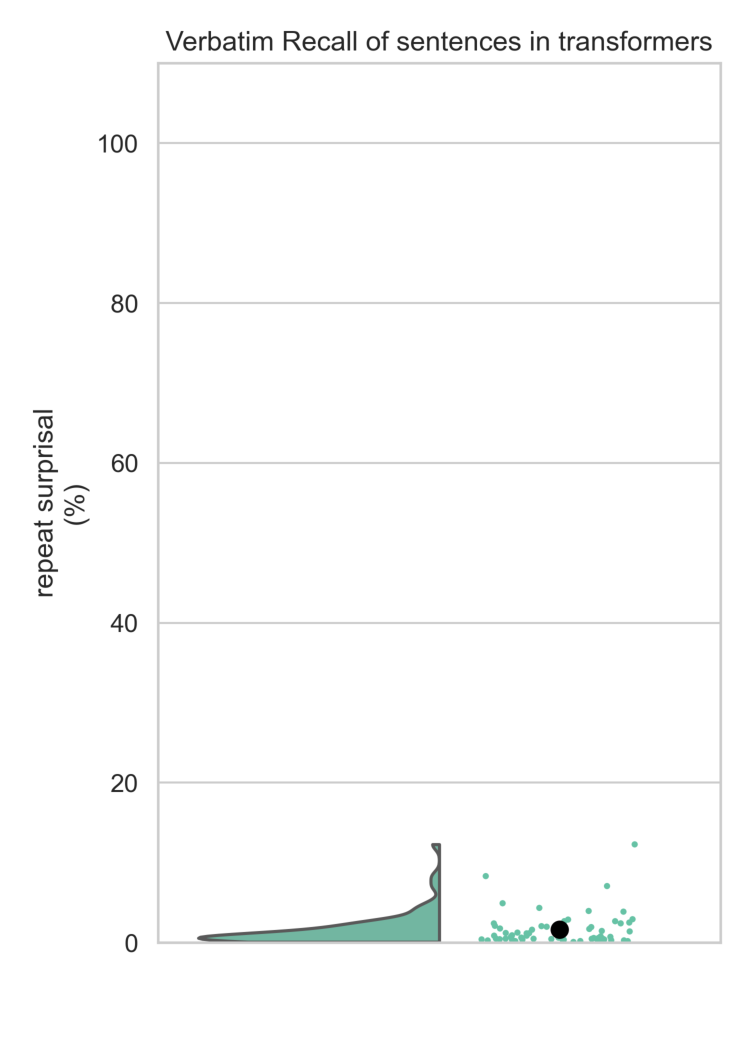
\includegraphics[width=0.5\textwidth]{experiments/repeat_surprisal_gpt2.pdf}
    \caption{Repeat surprisal of GPT-2 for verbatim repetition of sentences ($N = 60$). The Y axis shows the repeat surprisal as percentage. The ``raincloud plot'' \parencite{allen_raincloud_2019} shows the distribution of repeat surprisal as kernel density estimate (left). The points (right) are the actual repeat surprisal values for each measure. The black point (right) indicates the mean. Bootstrap $95\%$ confidence intervals are plotted around the mean, but are not visible due the consistency of the repeat surprisal in this experiment.}
    \label{fig:repeat_gpt2}
\end{wrapfigure}


\subsubsection{Interim Discussion}
The results show that transformers are able to perform verbatim recall for sentences.
This generalizes the finding that transformers can recall lists of arbitrary nouns.
Still, this experiment does not help us to differentiate between different concept-models: Any concept-model can explain this pattern of results (see \ref{app:repeat_null_explanation}).


\subsection{Word-swap experiment: Differentiating the concept-models} \label{exp:word_swap}

In order to characterize what relationships of the sentences are captured by the transformers fWM, we distinguish between four possible concept-models (see Section \ref{sec:expectations}).
In order to do that, we ran an experiment in which the results for each concept-model come apart:
In this experiment we introduce three conditions which differ by how a target word in the test sentence is swapped in the test sentence.
We then measure the repeat surprisal of that target word, and try to determine which of our concept-models best fits to our results.


\subsubsection{Experimental Setup}

We test the transformer across three conditions within our paradigm. Different from the Repeat experiment, we focus our analysis on repeat surprisal of single-tokens. The conditions only differ at the position of a verb or noun within the test-sentence of both the Test-sequence and Control-sequence.

Specifically, the first condition (\textit{repeat} - RPT) repeats the word from the encoding-sentence at the same position in the test-sentence.
The second condition (\textit{synonym} - SYN) swaps the original target word with a synonym\footnote{For details of synonym sampling see \ref{app:syn_sampling}} of the original target word.
The third condition (\textit{arbitrary} - ARB) swaps the original target word with an arbitrary word which is within the same part-of-speech (POS) category as the target-word (e.g. a noun is swapped with an arbitrary noun).

For instance, we take a measure defined by the prefix, the encoding-sentence ``A proposal to rename the species cannot be carried through.'', an intervention, and the (repeated) test-sentence ``A \textbf{proposal} to rename the species cannot be carried through.''. We mark the position of the target noun ``proposal''. Now, we measure the repeat surprisal at the position of \textbf{proposal} in the test-sentence for each condition. In RPT, proposal is repeated, in SYN proposal is swapped with a synonym (e.g. ``bid'', ``motion'', ``proposition''), and in ARB proposal is swapped with an arbitrary word within the same part-of-speech category (e.g. ``view'', ``charge'', ``microphone''). For details, see Figure \ref{fig:word_swap_setup} and \ref{app:word_swap_setup}.

Repeat surprisal is computed by selecting the surprisal value of the target noun/verb. Formally, $f_\text{sel} = \left(\left\{\left(w_1, s(w_1)\right), \dots \right\}\right) = \sum_i \delta_{w_i} s(w_i)$ where $\delta_{w_i}$ is $1$ if $w_i$ is the target word and $0$ elsewhere. We then can compute the $\texttt{repeat surprisal}_{f_\text{sel}}$ with eq. \ref{eq:repeat_surprisal}.

\subsubsection{Hypotheses} \label{sec:expectations}
Depending on which concept-model the fWM of the transformer is closer to, we expect different results across the three conditions:


\paragraph{M0: Indiscriminate}

The indiscriminate fWM increases the probabilities of previously seen words regardless of where in context they occur.
Accordingly, the target word in the Test-sequence does appear in prior context, and is assigned low surprisal values.
On the other hand, the target word in the Control-sequence in the RPT condition should be assigned a large surprisal value, as it does not appear in prior context and the transformer does not form an expectation for it.
Importantly, the repeat surprisal for target words in the RPT condition cannot be too low -- the indiscriminate WM has to distribute its probability mass over all tokens in prior context.
Subsequently, repeat surprisal values in RPT consistent with M0 are low but not $0\%$.
In the SYN and ARB conditions, an indiscriminate WM mechanism would neither expect the target word in the Test-sequence, nor in the Control-sequence (as synonyms and arbitrary tokens do not occur in context).
Hence, the repeat surprisal for ARB and SYN should be close to $100\%$.

\paragraph{M1: Plain copy-paste}
A plain copy-paste mechanism is only able to predict words which were in previous context.
In contrast to M0, under M1 the model only assigns high probabilities to one word: the exact word that followed the currently processed word.
Because the model is expecting the exact token (i.e. probability mass is concentrated on one token), repeat surprisal in RPT is expected to be $0\%$, or minimally above it.
In the SYN and ARB conditions, similarly to M0, the plain-copy-paste mechanism would neither expect the target word in the Test-sequence nor in the Control-sequence.
Hence, repeat surprisal values in ARB and SYN conditions consistent with M1 should be close to $100\%$.

\paragraph{M2: Lexical-Syntactic copy-paste}
The lexical-syntactic copy-paste mechanism allows the model to predict words within the same syntactic class.
It is expected that such a mechanism leads to repeat surprisal below $100\%$ in RPT, ARB and SYN: a repeated word RPT and a semantically similar SYN are within the same syntactic class to the original word.
Moreover, the word swap in ARB is defined over words with the same POS-category. In contrast with the plain-copy-paste mechanism where probability mass is centered on one token, the repeat surprisal in M2 should be significantly over $0\%$, as such a mechanism would distribute the probability mass over big parts of its vocabulary (e.g. all nouns).

\paragraph{M3: Word-Semantic copy-paste}
The Word-Semantic copy-paste mechanism allows for prediction of semantically similar words.
Again, such a model is expected to spread the probability mass over multiple words.
Thus, RPT is assumed to be lower than $100\%$, but not exactly $0\%$.
Furthermore, as the synonyms of the SYN condition are within the semantically similar words predicted by this model, repeat surprisal for SYN is expected be lower than $100\%$.
On the other hand, the target words in the ARB condition are very likely not semantically related to the encoding-sentence.
Hence, repeat surprisal values consistent with M3 should not be lower than $100\%$ in ARB.

\begin{figure}
    \centering
    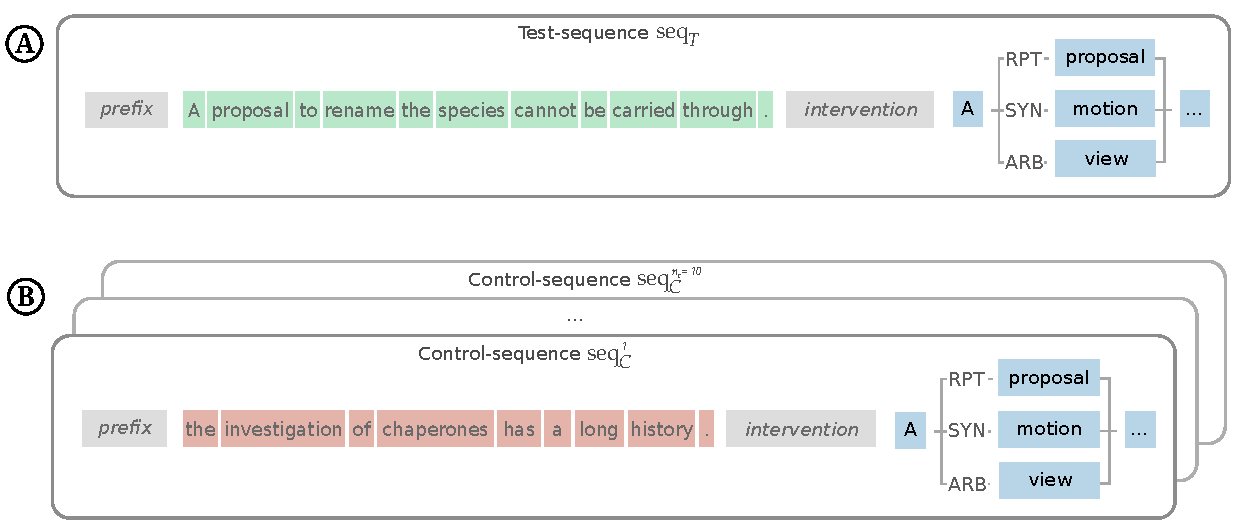
\includegraphics[width=\textwidth]{methods/word_swap_setup.pdf}
    \caption{Experimental setup for the word-swap experiment. \textbf{A}: Test-sequence for the three word swap conditions. Prefix, encoding-sentence and intervention are identical to the previous experiment. In the test-sentence, the target word ``proposal'' is either repeated (RPT), swapped with a synonym (SYN) or swapped with an arbitrary word within the same POS-category (ARB). \textbf{B}: Control-sequence for the three word swap conditions. }
    \label{fig:word_swap_setup}
\end{figure}

\subsubsection{Results}\label{ex:2_word_swap_results}

The results are visualized in Figure \ref{fig:word_swap_experiment}. Results for all transformers can be found in \ref{fig:word_swap_all}.

\paragraph{RPT}
With an average repeat surprisal for nouns of $6.8\%$ and a median of $3.1\%$ values are close to $0\%$. This means that surprisal values for the target words in the T-sequences are on average $6.8\%$ to the surprisal of target words in the C-sequences. Repeat surprisal for verbs is comparable, albeit slightly lower: the mean for verbs is $4.33\%$ and the median is $1.47\%$.

\paragraph{SYN}
The average repeat surprisal for nouns is $74.24\%$ and the median is $70.44\%$. The $95\%$ confidence interval lies well below a repeat surprisal of $100\%$. This cannot be said for verbs. With a mean of $101.14\%$ and a median of $92.21\%$ the repeat surprisal measurements are close to $100\%$. Moreover, as observable in \ref{fig:word_swap_experiment} the  $95\%$ confidence interval does not entirely lie below $100\%$.

\paragraph{ARB}
Both mean and median for verbs ($122\%$/$112.58\%$) and nouns ($128.41\%$/$120.87\%$) are well above $100\%$. This also applies to the confidence-intervals.


\begin{figure}
    \centering
    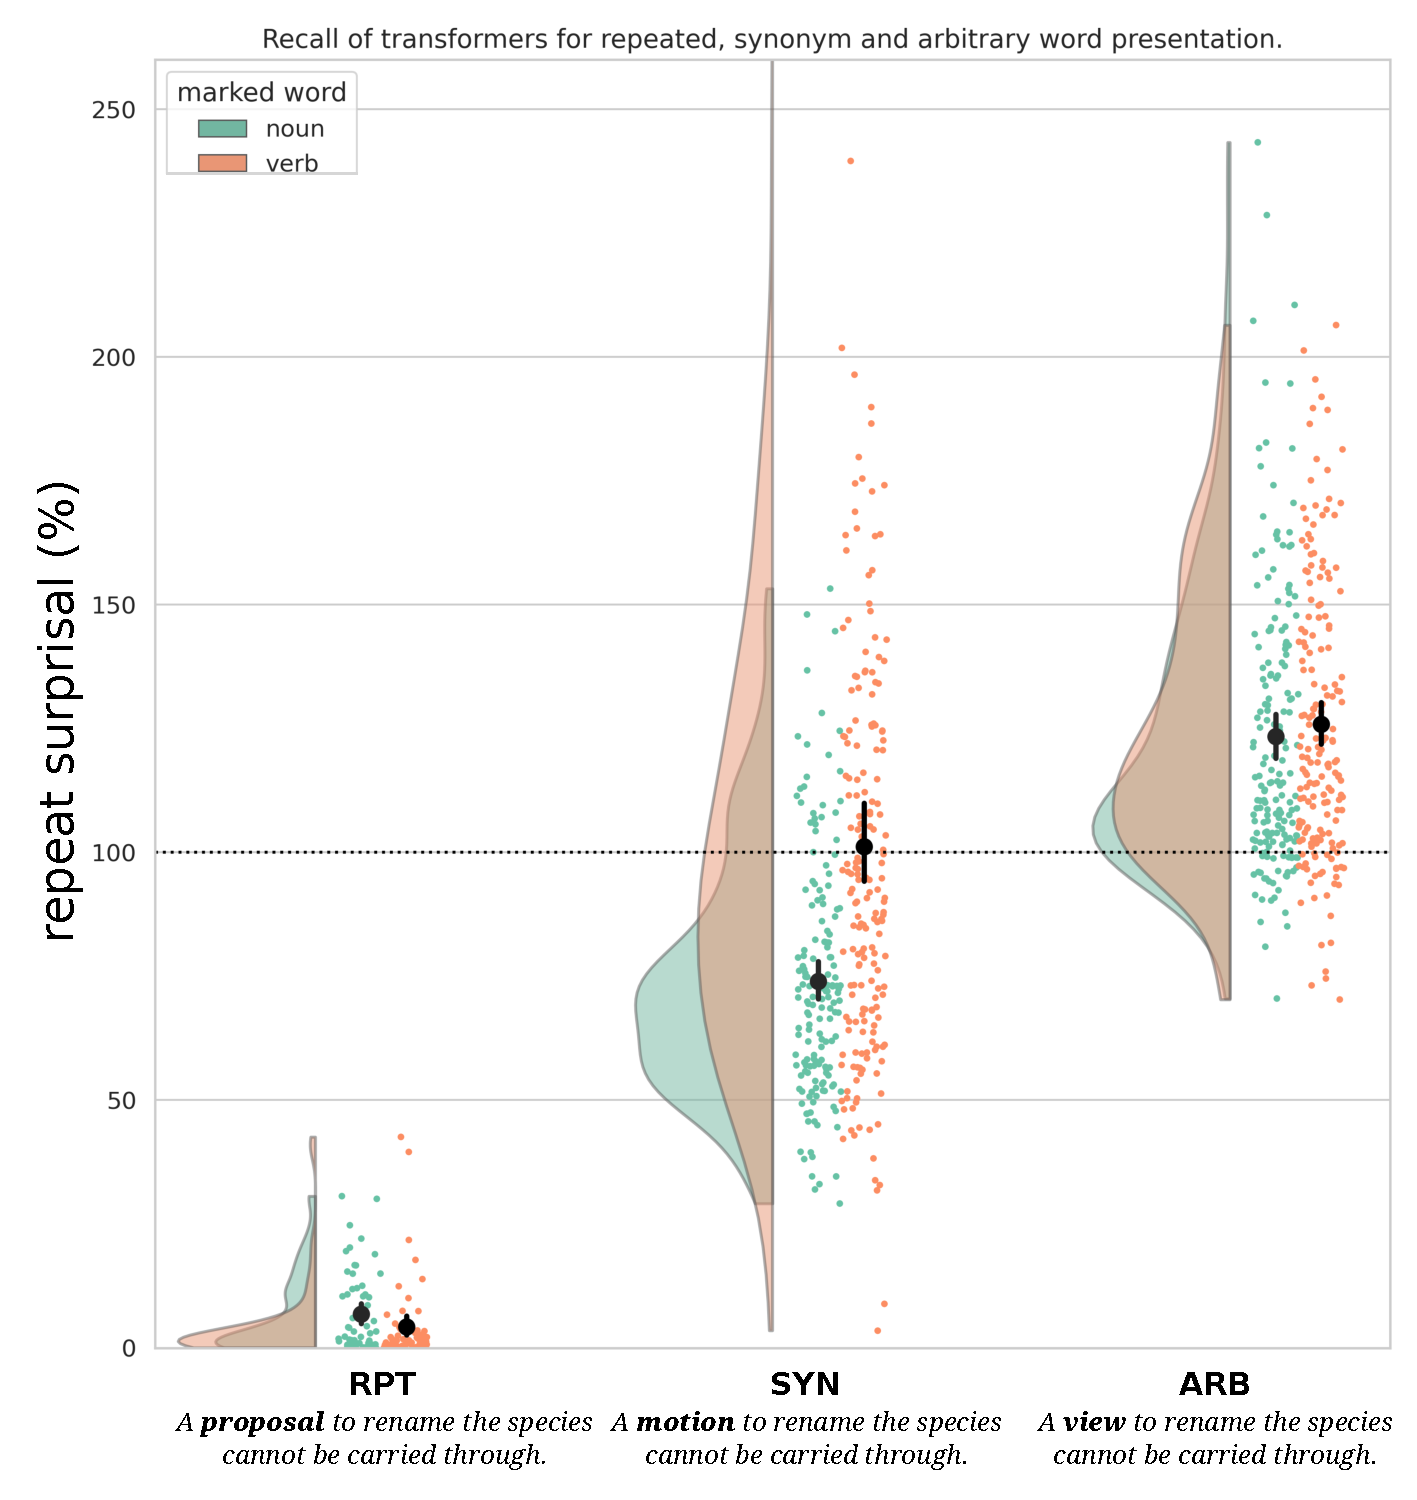
\includegraphics[width=\textwidth]{experiments/word_swap_plot.pdf}
    \caption{Raincloud plot of repeat surprisal for the RPT, SYN and ARB conditions in the word swap experiment. Given the encoding sentence "A proposal to rename the species cannot be carried through." an example test sentence with the swapped word marked is pictured below the condition labels. The results for nouns are pictured in green, the results for verbs in orange. The leftmost element shows the distributions of measurements, whilst the scatter plots show the actual repeat surprisal for every measure. The black point indicates the mean, the whiskers denote the $95\%$ confidence interval. Notice that that there are different numbers of data points per condition. Still, a clear difference between the conditions is visible.}
    \label{fig:word_swap_experiment}
\end{figure}

\subsubsection{Interim Discussion}

The word-swap experiment suggests the transformer is not employing a model such as the indiscriminate fWM M0. Although the results of the RPT condition are consistent with predictions of M0, the repeat surprisal in the ARB and SYN conditions is not centered around $100\%$.
This means the transformer is extracting information from the encoding-sentence for the prediction of tokens in the test-sentence, irrespective of the fact that the word in the test-sentence never occurred in prior context, invalidating M0.
Furthermore, the lexical-syntactic copy-paste fWM M2 also seems to be readily rejected: the results for ARB indicate that the model does not assign probabilities to all words within the same syntactic category.
On the contrary, with repeat surprisal mostly over $100\%$, the transformer is actively increasing surprisal of words within the same POS-category after the presentation of the repeated encoding-sentence.

The plain copy-paste fWM M1 seems to be a promising candidate describing the transformer fWM during sentence repetition.
The consistently low repeat surprisal values in the RPT condition strongly speak in favor of a mechanism comparable to M1.
Still, a mechanism such as M1 could not account for the results in SYN, especially not for the results regarding the nouns, as it would only predict the tokens that occur in context which is not guaranteed for synonyms.

Lastly, the word-semantic copy-paste fWM M3 seems to be most consistent with the results. The slightly reduced repeat surprisal for synonyms shows that transformers fWM indeed use the encoded information to predict semantically related words. Furthermore, it is conceivable that most of the weight is put into the verbatim repetition, as it is deemed as ``best synonym''.

We have to keep in mind the limit of this experimental design.
Since sampling of words within synonyms is not exhaustive, we may just have missed the right target words in the SYN condition on which the transformer shows a more pronounced effect.
The transformer might only have learned a subset of the targets we tested it on.
Even though this subset might not reflect human-level knowledge, it still remains relevant whether the the transformers' fWM can be characterized as a word-semantic copy-paste fWM M3 model operating on a subset synonyms.

The only condition in which results from nouns and verbs vary is the SYN condition. The result for nouns strongly speaks for the fWM of transformers being sensitive towards synonyms. On the other side, the results for verbs would suggest that the model is not sensitive at all towards synonyms for verbs. A plausible explanation for the lack of effect on verbs in SYN could be the general observation that nouns have more synonyms than verbs. Another hypothesis takes into account the placement of nouns and verbs within the sentence: whereas the median noun position within our sentences is the third position, the median verb position is the ninth. A position further along the test-sentence might lead to a stronger expectancy of the verbatim repetition, as the matched context sequence is longer. This could then result in less surprisal reduction for synonyms.

\subsection{Probability Change Analysis}\label{ex:3_prob_change_analysis}

To account for the shortcomings of the Word swap experiment, we introduce a third experiment: the probability change analysis.
Instead of analyzing the repeat surprisal on specific target words, we analyse the top six words in the transformers' output probability distribution which receive the highest change in probability after the presentation of the encoding-sentence in context.
By measuring the change of word probability given an encoding-sentence (relative to to a control-sentence) we can determine which words in the vocabulary are most influenced by the presence of the encoding-sentence.
In other words, we can have a direct look at the transformer fWM effect.
In turn, by analyzing the words that changed the most, we may determine -- in conjunction with the results from our first experiment -- which concept-model may provide the best account of fWM during sentential repetition.


\subsubsection{Experimental setup}
Similar to the word-swap experiment, the probability change analysis only focuses on the target word: a specific noun or verb within the test-sentence.
But instead of measuring the repeat surprisal of predetermined words, the probability change analysis measures the probability of all words in the vocabulary at the position of the target word in the sentence.

We first measure the output probability distribution over all words at the target word position in the Test-sequence (i.e. when the test-sentence has a relationship to the encoding-sentence in context).
We then do the same for target word position in the C-sequences (i.e. when the test-sentence has no relationship to the control-sentence in context).
We generated 10 control sequences.
We compute the average probability distribution in the 10 sequences to get an estimate of the probability for each word in the vocabulary at the target word position.

We can now measure the \textit{change in probability} between the probability distribution at the target word in the Test-sequence and the average probability distribution at the target word of the Control-sequences.
This is a direct measurement of the change in probability a transformer assigns a word when presented with a context which stands in a relationship with the test-sentence versus a context which does not stand in a relationship to the test-sentence.

The experiment was run for GPT2-base, with $60$ sentences (section \ref{met:sentences_used}).
For each sentence, the six predictions with the biggest probability change are analyzed and categorized by hand.
In total $360$ predictions were categorized both for nouns and verbs.

\begin{figure}
    \centering
    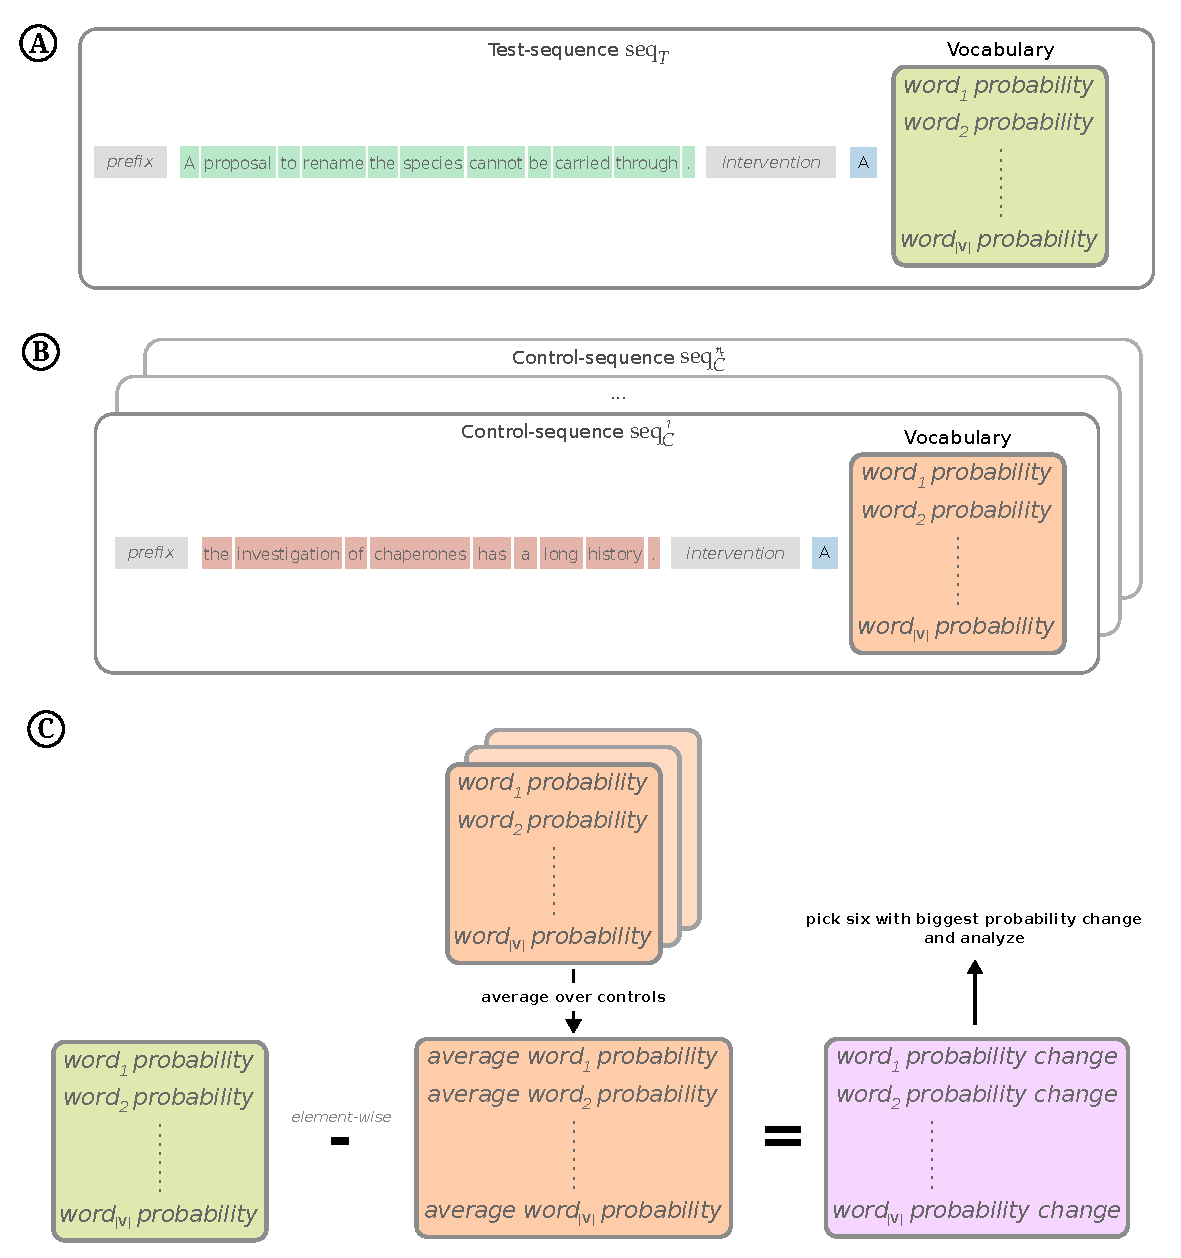
\includegraphics[width=\textwidth]{methods/prob_change_setup.pdf}
    \caption{Experimental setup for the probability change analysis. \textbf{A}: In the Test-sequence we record probabilities of all words within the vocabulary (green) after presentation of prefix (grey), encoding-sentence (green), intervention (grey) and the start of the test-sentence (blue). \textbf{B}: In the Control-sequences we record probabilities of all words within the vocabulary (orange) after presentation of prefix, control-sentence (red), intervention (grey) and the start of the test-sentence (blue). \textbf{C}: Probabilities of words from the Control-sequences are averaged, and then subtracted with the probabilities of the words from the Test-sequence to obtain the probability change for each word in the Vocabulary (purple). The six words which have the biggest positive probability change are analyzed.}
    \label{fig:prob_change_experiment}
\end{figure}

\subsubsection{Results}

\begin{table} \centering
\scalebox{0.9}{
\begin{tabular}{c c c c c c c c}
\hline
\multicolumn{8}{l}{{\cellcolor{gray!25}\small Sentence}}\\
\thead{target noun} & \thead{probability\\in test-\\sequence} & \thead{\#1} & \thead{\#2} & \thead{\#3} & \thead{\#4} & \thead{\#5} & \thead{\#6} \\
\hline\hline
\multicolumn{8}{p{1.08\linewidth}}{\cellcolor{gray!25}the section on current routes adds nothing to the info .}\\
\thead{\footnotesize section\\} &\thead{\footnotesize 0.629} & \colorbox[rgb]{0.59, 0.78, 0.64}{\thead{\footnotesize section\\(0.6284)}} & \colorbox[rgb]{1.0, 1.0, 0.0}{ \thead{\footnotesize paragraph\\(0.0131) \hfill}} & \colorbox[rgb]{1.0, 0.75, 0.0}{\thead{\footnotesize sections\\(0.012) \hfill}} & \colorbox[rgb]{1.0, 1.0, 0.0}{\thead{\footnotesize page\\(0.0089)}} & \colorbox[rgb]{1.0, 1.0, 0.0}{\thead{\footnotesize part\\(0.0079)}} &\colorbox[rgb]{0.6, 0.4, 0.8}{\thead{\footnotesize route\\(0.0077)}} \\
\hline
\multicolumn{8}{p{1.08\linewidth}}{\cellcolor{gray!25}the base of the buildings contains commercial space , including two restaurants , a dental office ( pinnacle dental ) , a medical clinic , and spa , while the surrounding area will consist of public parks , shops and recreation spaces .}\\
\thead{\footnotesize base\\} &\thead{\footnotesize 0.424} & \colorbox[rgb]{0.59, 0.78, 0.64}{\thead{\footnotesize base\\(0.4239)}} & \colorbox[rgb]{0.6, 0.4, 0.8}{\thead{\footnotesize building\\(0.0288)}} & \colorbox[rgb]{1.0, 0.75, 0.0}{\thead{ \footnotesize bases\\(0.017)}} &  \colorbox[rgb]{0.92, 0.3, 0.26}{\thead{\footnotesize location\\(0.0079)}} & \colorbox[rgb]{0.6, 0.4, 0.8}{\thead{\footnotesize area\\(0.0076)}} & \colorbox[rgb]{0.6, 0.4, 0.8}{\thead{\footnotesize buildings\\(0.0065)}} \\
\hline
\multicolumn{8}{p{1.08\linewidth}}{\cellcolor{gray!25}the genetic variation among the viruses isolated from different places ( 7-8 ) increases the difficulty of developing vaccines against it .}\\
\thead{\footnotesize variation\\} &\thead{\footnotesize 0.919} & \colorbox[rgb]{0.59, 0.78, 0.64}{\thead{\footnotesize variation\\(0.9169)}} & \colorbox[rgb]{1.0, 1.0, 0.0}{ \thead{\footnotesize variance\\(0.0229)}} & \colorbox[rgb]{1.0, 0.75, 0.0}{ \thead{\footnotesize variant\\(0.0135)}} & \colorbox[rgb]{1.0, 0.75, 0.0}{\thead{\footnotesize variations\\(0.0133)}} &  \colorbox[rgb]{1.0, 1.0, 0.0}{ \thead{\footnotesize variability\\(0.0083)}} & \colorbox[rgb]{1.0, 0.75, 0.0}{ \thead{\footnotesize variants\\(0.0009)}} \\
\hline
\multicolumn{8}{p{1.08\linewidth}}{\cellcolor{gray!25}the edwardian semi-detached houses of brantwood road , facing the park have an art deco style whilst those in ashburnham road include ornate balconies .   }\\
\thead{\footnotesize houses} & \thead{\footnotesize 0.95} & \colorbox[rgb]{0.59, 0.78, 0.64}{ \thead{\footnotesize houses\\(0.9498)}} & \colorbox[rgb]{1.0, 1.0, 0.0}{ \thead{\footnotesize homes\\(0.0092)}} & \colorbox[rgb]{1.0, 0.75, 0.0}{\thead{\footnotesize house\\(0.0076)}} & \colorbox[rgb]{1.0, 0.75, 0.0}{\thead{\footnotesize \_houses\\(0.0016)}} & \colorbox[rgb]{1.0, 1.0, 0.0}{\thead{\footnotesize dwellings\\(0.0016)}} & \colorbox[rgb]{1.0, 1.0, 0.0}{\thead{\footnotesize places\\(0.0006)}} \\
\hline
\multicolumn{8}{p{1.08\linewidth}}{\cellcolor{gray!25}for protestant denominations , the purposes of marriage include intimate companionship , rearing children and mutual support for both husband and wife to fulfill their life callings .}\\
\thead{\footnotesize purposes} & \thead{\footnotesize 0.855} &  \colorbox[rgb]{0.59, 0.78, 0.64}{\thead{\footnotesize purposes\\(0.8546)}} & \colorbox[rgb]{1.0, 0.75, 0.0}{ \thead{\footnotesize purpose\\(0.1033)}} & \colorbox[rgb]{1.0, 1.0, 0.0}{ \thead{\footnotesize uses\\(0.0035)}} & \colorbox[rgb]{0.92, 0.3, 0.26}{\thead{\footnotesize ends\\(0.0034)}} & \colorbox[rgb]{0.92, 0.3, 0.26}{\thead{\footnotesize means\\(0.0025)}} & \colorbox[rgb]{1.0, 1.0, 0.0}{\thead{\footnotesize functions\\(0.0016)}} \\
\hline
\end{tabular}
}
\caption{Example data of the words with the biggest change in the probability change experiment. For each sentence, the target word is provided together with the model's absolute probability for the target word given the repeat context. The rest of the columns denote the words with highest probability change. The probability change is in the brackets below the word. Words the transformer predicted to be a continuation without a blank-space start with ``\_''. Colors mark error categories of the error analysis: \textit{Green}: Verbatim repetition; \textit{Yellow}: Semantically correct, syntactically correct; \textit{Orange}: Semantically correct, syntactically incorrect;  \textit{Red}: Semantically incorrect, syntactically corrrect; \textit{Purple}: Position shifted word; Other categories did occur in this subset.} \label{Tab:prediction_change}
\end{table}
% TODO: !

The first ten results for the experiment can be found in Table \ref{Tab:prediction_change}.
A clear pattern for the word with the highest probability change can be seen. Consistent with the findings of the previous experiment, it is almost always the verbatim repetition of the appropriate word in the encoding-sentence.
To draw more conclusions, we categorize each word of the top six words with the biggest positive change into eight categories.
These categories are determined manually by us based on the relationship of the word to the encoding-sentence in the context.
For instance, given the Test-sequence "[\textit{prefix}] the investigation of chaperones has a long history . [\textit{intervention}] the investigation of chaperones [???]" the prediction ``has'' in the position [???] is the verbatim repetition of the previous context, and ``have'' would be semantically correct, but syntactically wrong (subject-verb-disagreement).
We use following categories:\\
\textbf{Verbatim repetition}
A word that is the verbatim repetition of the word in the encoding-sentence (e.g. ``has'').\\
\textbf{Semantically correct, syntactically correct}
A word that is semantically and syntactically fitting -- in other words, a good synonym.
This category only includes words that preserve the meaning of the sentence, and words which allow the sentence to be continued as given in the encoding sentence (e.g. ``carries'').\\
\textbf{Semantically correct, syntactically incorrect}
A word which may semantically fit, but is syntactically wrong given the encoding sentence. For instance ``have'' with wrong subject-verb-agreement or ``had'' having the wrong tense.\\
\textbf{Semantically incorrect, syntactically correct}
A word which semantically does not fit, but is within the same POS-category with the repeated word (e.g. ``belongs'').\\
\textbf{Semantically incorrect, syntactically incorrect)}
A word which neither matches semantically nor syntactically (e.g. ``proudly'').\\
\textbf{Position shifted word}
A word which is predicted at a wrong sequence position -- it originally appeared in a different position of the encoding-sentence as the repeated word (e.g. ``long'').\\
\textbf{Other}
All words which cannot be categorized in the categories above.
For example, these may are single letter predictions such as ``C'' or in rare cases words which have appeared in the intervention\footnote{This happened exactly six times, but only in the noun condition.}.\\

The result of the categorization can be seen in Table \ref{Tab:prediction_change_analysis}.
For each category, the cumulative probability change percentage of all words within the category is shown alongside with the absolute category probability change.
The probability change percentage is computed by adding the probability change of each word within the category, obtaining the absolute category probability change.
This value is divided by the sum of the absolute category probability change of all categories, resulting in the cumulative probability change percentage.

The results show that the transformer given the repeat sentence context shifts the probability distribution mostly towards the verbatim repeated word from the context.
For nouns $89.51\%$ of probability change happens within the \textit{verbatim repetition} category.
For verbs, this effect is by $5\%$ stronger with $94.26\%$.

To ease the interpretation of the results we group both \textit{semantically correct} (second and third) categories: their probability change percentage together is $5.22\%$ and $4.43\%$ for nouns and verbs respectively.
Moreover, we group both \textit{syntactically correct} (second and fourth) categories, together they have a probability change percentage of $3.03\%$ and $3.56$ for nouns and verbs respectively.

Occurrences of words within categories mainly happen for the first four categories.
This is more so the case for verbs than for nouns, where a respectable amount of word occurrences resides in the ``position shifted word'' category.
For verbs, most occurrences are in the \textit{semantically correct, syntactically incorrect}-category $132$ occurrences.
For nouns, the maximal occurrences are in the \textit{semantically correct, syntactically correct}-category with $82$ occurrences.
Note that for both nouns and verbs in $58$ of $60$ sentences the verbatim repetition was present.
In the case of nouns, these were two sentences in which the noun was the first word of the sentence.

The difference in probability change between nouns and verbs mainly stems from an increase in probability change in the ``verbatim repetition'' category for verbs compared to nouns and a reduction of probability change in the categories ``position shifted word'' and ``other''.
In the \textit{semantically correct, syntactically correct}-category the transformer shows a higher probability change percentage for verbs than for nouns.

\begin{table} \centering
\begin{threeparttable}
\begin{tabular}{l | c c | c c}
\toprule
{} & \multicolumn{2}{c|}{\thead{nouns}} & \multicolumn{2}{c}{\thead{verbs}} \\
\thead{word category} &  \thead{cumulative probability-\\change percentage\\(absolute)} & \thead{occurrences} & \thead{cumulative probability-\\change percentage \\(absolute)} &  \thead{occurrences} \\
\midrule
\thead{verbatim repetition}                              &   89.51 (37.31) & 58 &  94.26 (47.12)  &  58 \\
\thead{semantically correct,\\syntactically correct}     &     1.5 (0.62)  & 82 &   2.58 (1.29)   &  83 \\
\thead{semantically correct,\\syntactically incorrect}   &    3.72 (1.55)  & 80 &   1.85 (0.92)   & 132 \\
\thead{semantically incorrect,\\syntactically correct}   &    1.53 (0.63)  & 70 &   0.98 (0.49)   &  54 \\
\thead{semantically incorrect,\\syntactically incorrect} &    0.65 (0.27)  & 16 &   0.24 (0.12)   &  17 \\
\thead{position\\shifted word}                           &    1.74 (0.72)  & 39 &   0.08 (0.04)   &   4 \\
\thead{other}                                            &    1.36 (0.57)  & 15 &   0.02 (0.01)   &   3 \\
\bottomrule
\end{tabular}
\caption{Categorization of the six words with the highest probability change in each sequence for verbs and nouns. We show the cumulative probability change percentage for each word category, together with the summed probability change within the category in brackets. This allows us to see how much probability change happens for each category -- in other words, which categories are affected the most by the encoding sentence in the context. The "occurrences" column shows the amount of times a word of the respective category appears within the top six predictions. As these are chosen irrespective of their actual probability change, the number of occurences cannot be attributed much importance.} \label{Tab:prediction_change_analysis}
\end{threeparttable}
\end{table}

\subsubsection{Interim Discussion}

Consistent with the findings of the previous experiment the highest probability change happens within the \textit{verbatim repetition}-category.
Moreover we find that the grouped \textit{semantically correct} categories have a .
The word-semantic copy-paste fWM M3 sets forth that synonyms of the continued word of the matched previous context are predicted.
Synonyms are semantically correct words independent of their syntactical correctness.
Hence, predictions within the \textit{semantically correct} categories are consistent with a word-semantic copy-paste fWM as posited in M3.
We can see that the second highest proportion of probability change just happens within these categories.
This further reinforces our previous discussion that a word-semantic copy paste fWM such as M3 approximates the transformers' fWM well.
Moreover, this confirms our prior hypothesis that we may have not probed the right subset of synonyms:
Although repeat surprisal in the syntactic word swap condition SYN of the previous experiment \ref{ex:2_word_swap_results} was close to $100\%$ and thus did not allow for a conclusive judgement, this experiment shows that $4.43\%$ of probability change lies within the \textit{semantically correct} category.
For that reason, the word-semantic copy paste fWM seems to approximate computational operations of transformer fWM for both nouns and verbs.

At a first glance, the probability change in the \textit{syntactically correct} categories would then by analogy hint towards a lexical-syntactic copy paste fWM M1.
In M1 probability is put into words which are within the same POS-category as the continued word of prior context.
But a lexical-syntactic copy paste mechanism would be expected to spread its probabilities over all or large proportion of words within a POS-category, and not a small subset.
The results of the within-POS-category word-swap condition ARB in the previous experiment \ref{ex:2_word_swap_results} show that the contrary is the case: in most cases the transformer fWM reduces the probability of words which are syntactically related, but semantically unrelated.
That does not mean that this happens for every word, which also can be seen in the previous experiment.
Thus, these results do not speak against the preliminary conclusions of the previous discussion, in which the lexical-syntactic copy-paste fWM was deemed to not approximate transformer fWM well.

An interesting observation concerns the difference in probability change percentages for nouns and verbs, especially when taking into account the amount of occurrences for each category.
Noticeably, in the \textit{semantically correct, syntactically incorrect}-category there are more occurrences for verbs, but a smaller probability change percentage than for nouns.
Analysis shows that these occurrences are mostly inflections of the verb (e.g. given "add", the inflections ``adds'' or ``added''). Their probability change percentage is so low, because they usually only occur when the model puts most of the probability change into the verbatim repeated word, without putting probability change into other synonyms.

Another observation is that probability change for the \textit{position shifted word} is almost only present for nouns.
This could be due to the much bigger availability of nouns within a sentence:
whereas our test sentence only have 1-2 verbs, they normally include multiple other nouns.
Thus there is just a higher amount of words the transformer fWM can confounded with the continued word of the matched prior context.

\newpage

\section{General Discussion}

\paragraph{Transformers show the ability of verbatim recall for sentences.} As seen with the repeat surprisal flooring at $0\%$ of the repeat experiment \ref{ex:1_repeat_results}, transformers -- independently of parameters and training corpus size -- show verbatim recall of sentences.
This generalizes the finding from Armeni et al. for noun-lists.
These results show a clear effect of fWM in transformers: previous context dynamically affects predictions only if that context stands in relation with the prediction.
In other words, the transformer has learned to store and retrieve sentences from context: part of the computational operations transformers can be described in terms of fWM.
This allows us to focus on determining which high-level descriptions characterize transformer fWM.

\paragraph{fWM of transformers during sentential repetition can be described by a a simple copy paste fWM which takes into account synonyms.}
The results of all three experiments are most consistent with the word-semantic copy-paste fWM (outlined in M3).
It describes a transformer fWM in which the longest possible previous context, which matches the  current context, is encoded and the probability for the word that followed the previous context is increased together with the probabilities for its synonyms.
At the same time, the transformer fWM puts a strong emphasis on the verbatim repetition of the word that occurred in the past context.
Because of that, transformer fWM is also well approximated by an even simpler copy-paste mechanism (outlined in M1) which only increases the probability for the repeated word in context and not the probability of synonyms into account.
But importantly, in the SYN condition of the word-swap experiment \ref{ex:2_word_swap_results} -- where target words on which we measure the effects of repetition are swapped with synonyms -- the results show that transformer fWM shows recall for synonyms, especially for nouns.
Furthermore, the cumulative probability change in experiment \ref{ex:3_prob_change_analysis} demonstrates directly that transformer fWM increases probabilities of words which are semantically related to the target word, albeit to a smaller extent than probabilities of exactly repeated words.
All in all, this provides compelling evidence that the computational operations in transformer fWM are characterized by a word-semantic copy-paste fWM which puts a high emphasis on the verbatim repetition of the continued word of matched previous context, but clearly spreads the retrieval computation over the semantically related words (synonyms) as well.

\paragraph{fWM effects are consistent across model and training corpus size.} The models investigated have vastly different numbers of parameters and are trained on different corpus sizes (Table \ref{Tab:models_used}).
This is also reflected in their perplexity on the test-set of the wikitext103 dataset.
Still, the transformer fWM effects are consistent. The lack of a significant difference e.g. in the SYN condition (target word swapped with a synonym) of the word swap experiment \ref{ex:2_word_swap_results} speaks towards our characterization of fWM being independent on architecture and training paradigm.

\paragraph{} The main contribution of this thesis is the development of the paradigm in order to characterize high-level computational operations in transformers.
This kind of understanding by using well-controlled behavioral paradigms to test how computational systems perform specific computations has a long history in human memory research \parencite{oberauer_benchmarks_2018}.
In contemporary computer science, and natural language processing specifically, experimental and empirical work provides and important toolkit for understanding the content of learned model representations.
But a growing body of work trying to understand transformers \parencite{rogers_primer_2020} demonstrates how hard it is to derive interpretable descriptions of these internal computational operations.
We think it may prove fruitful for researchers in natural language processing and computational linguistics to adopt methodologies used by psychologists, neuroscientists and cognitive scientists such as Marr's three levels of explanation \parencite{marr_vision_1982}, or in this case the WM framework in human memory research \parencite{baddeley_working_2003}.
By using the concept of functional Working Memory as an algorithmic description of transformer computations, we hope to give a glimpse into the possibilities of the approach.
This paradigm still offers a multitude of possible experiments and ways to explore fWM in transformers.
This possibly becomes even more interesting and relevant with improvements to transformers, as these improvements may allow for a more direct comparison to human WM.


\subsection{Future Work}

\paragraph{Concept-model refinement} For an improved matching of concept-model descriptions with the actual output of transformers a future continuation of this work could be the refinement of the concept-models.
For example, current descriptions of concept-models only take into account the encoding of the exact match of previous words and its next word.
It is a plausible alternative that not only this exact match is encoded, but also other words preceding the exact match.
This could be tested with test-sentences which consist of exactly the same words right until the target word. This target word then is a homonym, a word with multiple meanings, but preserved spelling (e.g. ``bank'': ``river bank'' and ``bank'' as institution), in which the meaning only becomes discernible through the context after the target word.

\paragraph{Additional experiments within the paradigm.} There are several interesting experimental setups to explore within this paradigm.
For example, given multiple encoding sentences it would be interesting to investigate whether encoding-sentences compete for retrieval and which of the encoding-sentences would be preferred.
Furthermore, it would be interesting to examine the effect of ``distracting'' words within the intervention.
In addition, the effect of differences within the intervention and prefix, shuffling and ordering characteristics of sentences, and the effect of syntactic properties of sentences remain to be explored.
Lastly, paraphrasing the encoding sentence to create a test-sentence which contains different words but retains the meaning of encoding-sentence, would allow to investigate the semantic encoding abilities of transformer fWM.
Brief experiments show that the model indeed is less surprised if the encoding-sentence is a paraphrase, although this effect seems to be mediated by the amount of shared words between paraphrases as opposed to shared abstract meaning.
Nevertheless, it would be interesting to characterize which levels of meaning the transformer fWM can capture in this ``repeated meaning'' experiment.

\paragraph{Generalization to non-repeated sentences.} For a more general characterization of transformers fWM, it would be of major interest to investigate the fWM when the test-sentence is not a repetition of the encoding-sentence.
For example, an experiment investigating fWM in such a manner could use textual entailment statements \parencite{dagan_pascal_2006}.
Can a transformer encode the information from the \textit{premise} to be less surprised at the presentation of the \textit{hypothesis}?
Compared of training a classifier for textual entailment, our paradigm would allow for a direct, non-fine-tuned analysis of transformer entailment performance, whilst providing the possibility for a more fine-grained analysis of results instead of only the usual three categories ``entailment'' or ``non-entailment''.
Again, such experiments will become more relevant with the advances of transformer capacities:
The effort to design such an experiment might not be worth it yet if it can be shown that current transformers use simple heuristics, like lexical overlap \parencite{mccoy_right_2019}.
On the other hand, such an experiment has the potential to uncover the processes in transformers which would speak for employment of more fine-grained computational operations.

\paragraph{Implementation of concept-models in transformer parameters} The algorithmic descriptions of transformer computations are detached from their implementational reality.
Given that we are content with our computational-algorithmic description, an interesting line of work would be to ``reverse engineer'' the implementation of such an algorithmic description in terms of transformer parameters.
This then may allow the attribution of certain roles to certain sets of parameters, which is an important aspect of understanding neural networks \parencite{mccloskey_networks_1991}.
Furthermore, the initialization of a transformer with such a pattern might prove to be a useful strategy for reducing the pre-training time.

\paragraph{Comparison of fWM to human WM.} The description of computational operations within transformers as fWM creates an avenue to compare the processes within transformers to processes within humans.
For instance, it may be possible to compare transformers in our paradigm to WM in a set of WM benchmarks introduced by \textcite{oberauer_benchmarks_2018}.
Such a comparison would be fruitful both for engineers as well as for psychologists, because it is thought that WM is an essential mechanism underpinning thought and higher cognition \parencite{baddeley_working_2003}.
Hence, the comparison may reveal deciding aspects which distinguish transformer fWM and human WM.

For example, the drop in recall performance with increased set size, is a benchmark finding that any model of human WM must account for \parencite{oberauer_benchmarks_2018}. Preliminary results show that transformers do not exhibit the set size effect during sentential repetition: in contrast to human WM, the performance of transformer fWM does not decrease with an increased set size.
This points towards a fundamental difference in human WM and transformer fWM, and raises questions such as e.g. do transformers need more explicit representations for single items and sets?

\newpage

% !TeX encoding = UTF-8


\section{Conclusion}

In this thesis, we have investigated the ability of transformers to recall sentences from past context. We refer to such  computational operations of transformers as ``functional Working Memory''.
The main contribution of the thesis is the development of the paradigm for testing functional working memory, in which transformer recall is measured by comparing surprisal levels in a sentence preceded by related and unrelated context.
We show that our paradigm allows us to measure transformer functional working memory. Specifically,  transformer retrieve verbatim repetitions of sentences and, to a smaller extent, broader semantic features of words in encoded sentences.
We further show that the transformer functional Working Memory is best described by a simple copy-paste mechanism which also takes into account synonyms of the verbatim copied word.
This effect is consistent across multiple models and training corpus sizes.
Our results show that it may be possible to describe certain computational operations within transformers on a conceptual algorithmic level.
This description of computational operations provides the opportunity to bridge the literature on human working memory research in order to understand computational operations in transformers.
By exploring the multitude of open avenues to continue this line of research, it remains to be seen whether this paradigm is a fruitful approach to study transformers. Furthermore, future work should focus on further refining the algorithmic descriptions developed in this thesis in order to test whether these are theoretically useful characterizations of computational operations in transformers.

\newpage


\printbibliography

\appendix
% !TeX encoding = UTF-8
\section{Appendix}


\subsection{Example Nonce Sentences}\label{ap:nonce_sentences}

\begin{table}[H] \centering
    \begin{threeparttable}
        \begin{tabular}{ p{0.66\linewidth} c c }
            \hline
            \thead{Sentence} & \thead{Noun} & \thead{Verb} \\
            \hline\hline
            the section on current routes adds nothing to the info . & section & adds \\
            the base of the buildings contains commercial space , including two restaurants , a dental office ( pinnacle dental ) , a medical clinic , and spa , while the surrounding area will consist of public parks , shops and recreation spaces . & base & contains \\
            the genetic variation among the viruses isolated from different places ( 7-8 ) increases the difficulty of developing vaccines against it . & variation & increases \\
            the list of shipwrecks in 1980 includes all ships sunk , foundered , grounded , or otherwise lost during 1980 . & list & includes \\
            the edwardian semi-detached houses of brantwood road , facing the park have an art deco style whilst those in ashburnham road include ornate balconies . & houses & have \\
            for protestant denominations , the purposes of marriage include intimate companionship , rearing children and mutual support for both husband and wife to fulfill their life callings . & purposes & include \\
            the signs , due to being the same colour green as the shield , show a green sign with a white inlay border , and a green outer border . & signs & show \\
            the application of these techniques to humans creates moral and ethical concerns in the opinion of some , while the advantages of sensible use of selected technologies is favored by others . & application & creates \\
            under chairwoman agnes gund , the moma ps1 's board of directors includes the artists laurie anderson and paul chan , art historian diana widmaier-picasso , fashion designer adam kimmel , and art collectors richard chang , peter norton , and julia stoschek . & board & includes \\
            \hline
        \end{tabular}
        \caption{First ten sentences from the nonce dataset.} \label{Tab:nonce_sentences}
    \end{threeparttable}
\end{table}

\clearpage


\subsection{Stabilization of repeat surprisal with 10 control sequences}\label{app:rs_10_controls}

\begin{figure}[H]
  \centering
  \subfloat[\centering average surprisal by amount of control sequences for 50 randomized trials.]{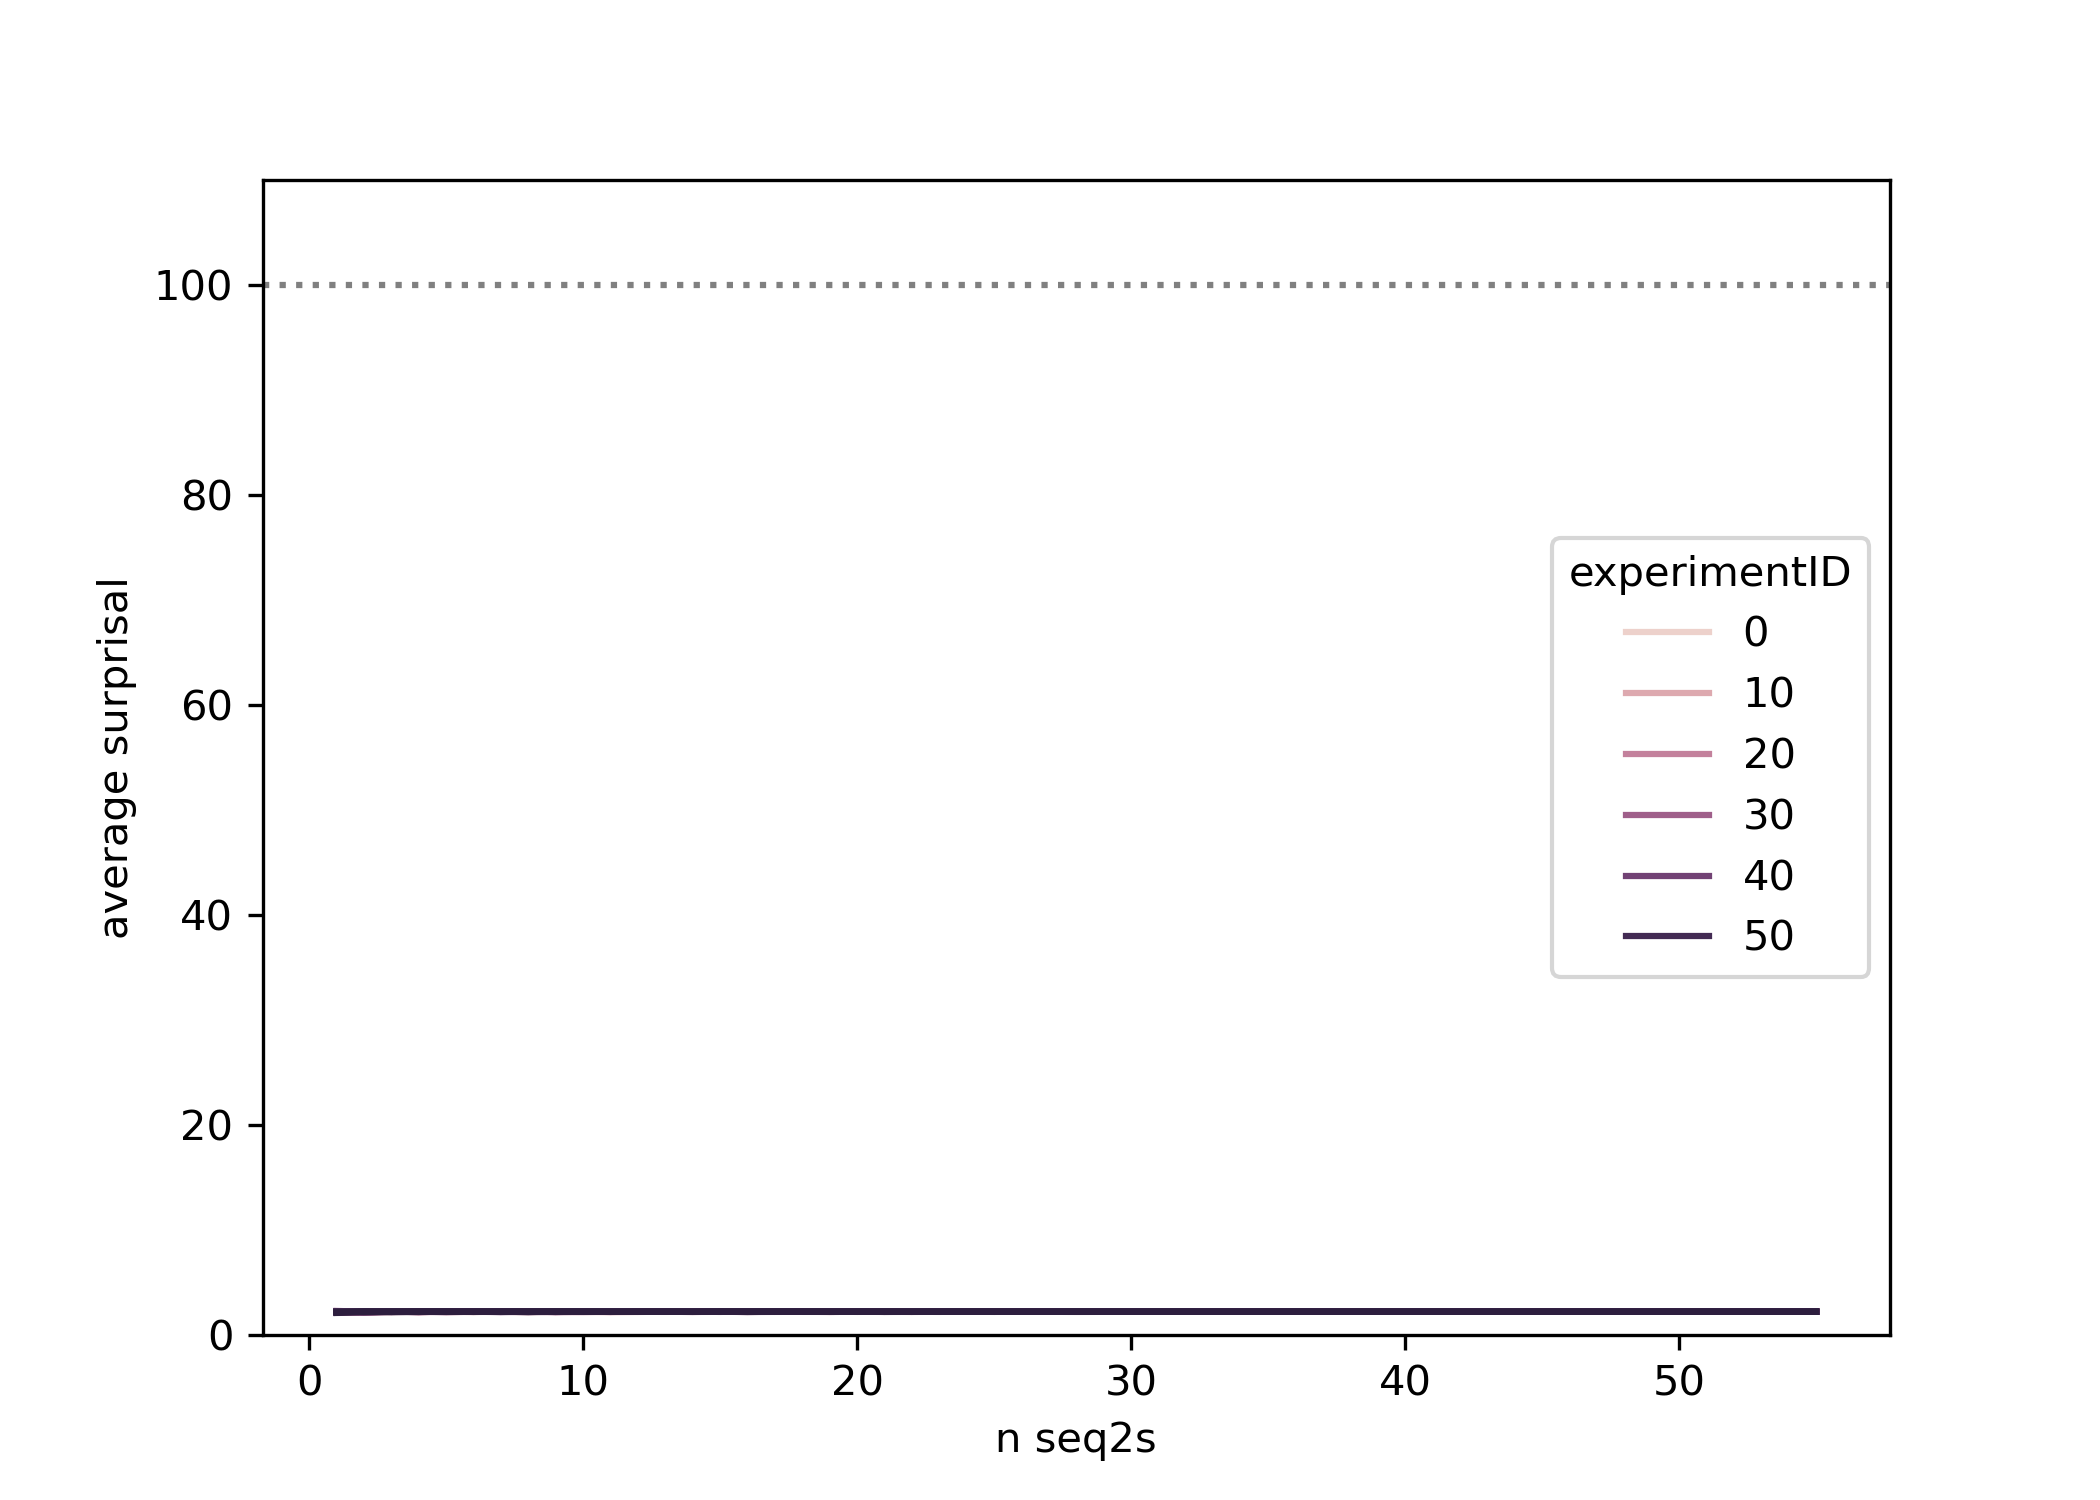
\includegraphics[width=.4\textwidth]{appendix/surprisal_nseq2.png}}\quad
  \subfloat[\centering same as (a), but scaled y-axis (surprisal) range to 2-2.4 bits]{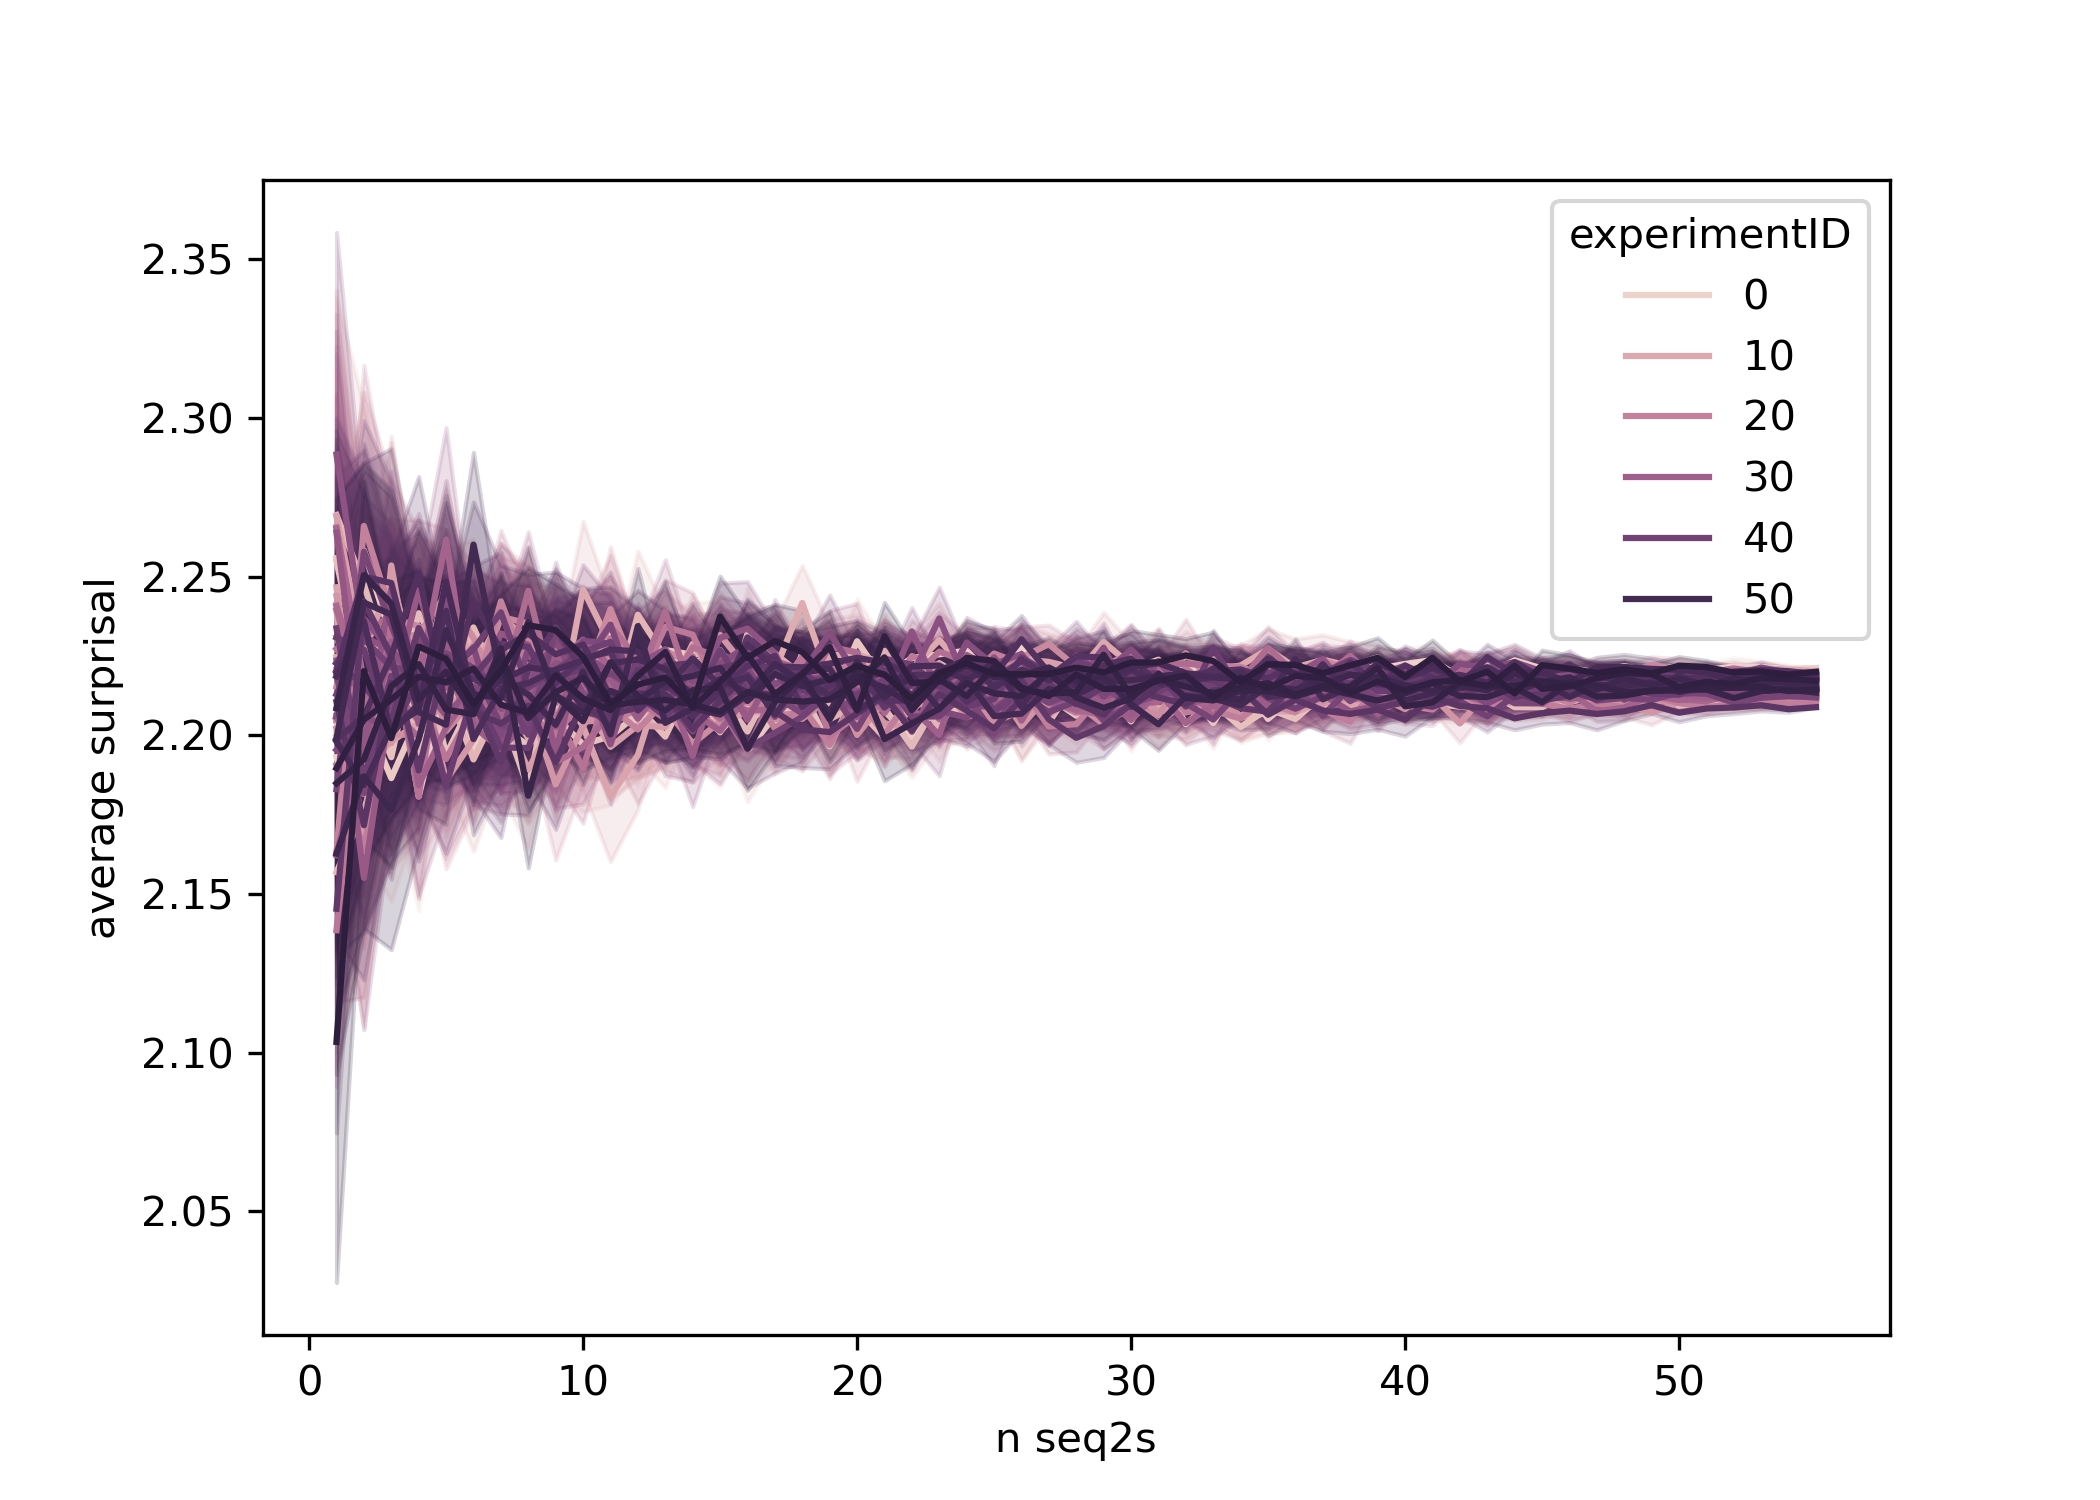
\includegraphics[width=.4\textwidth]{appendix/surprisal_nseq2_closeup.png}}\\
  \subfloat[average repeat surprisal by amount of control sequences for 50 randomized trials.]{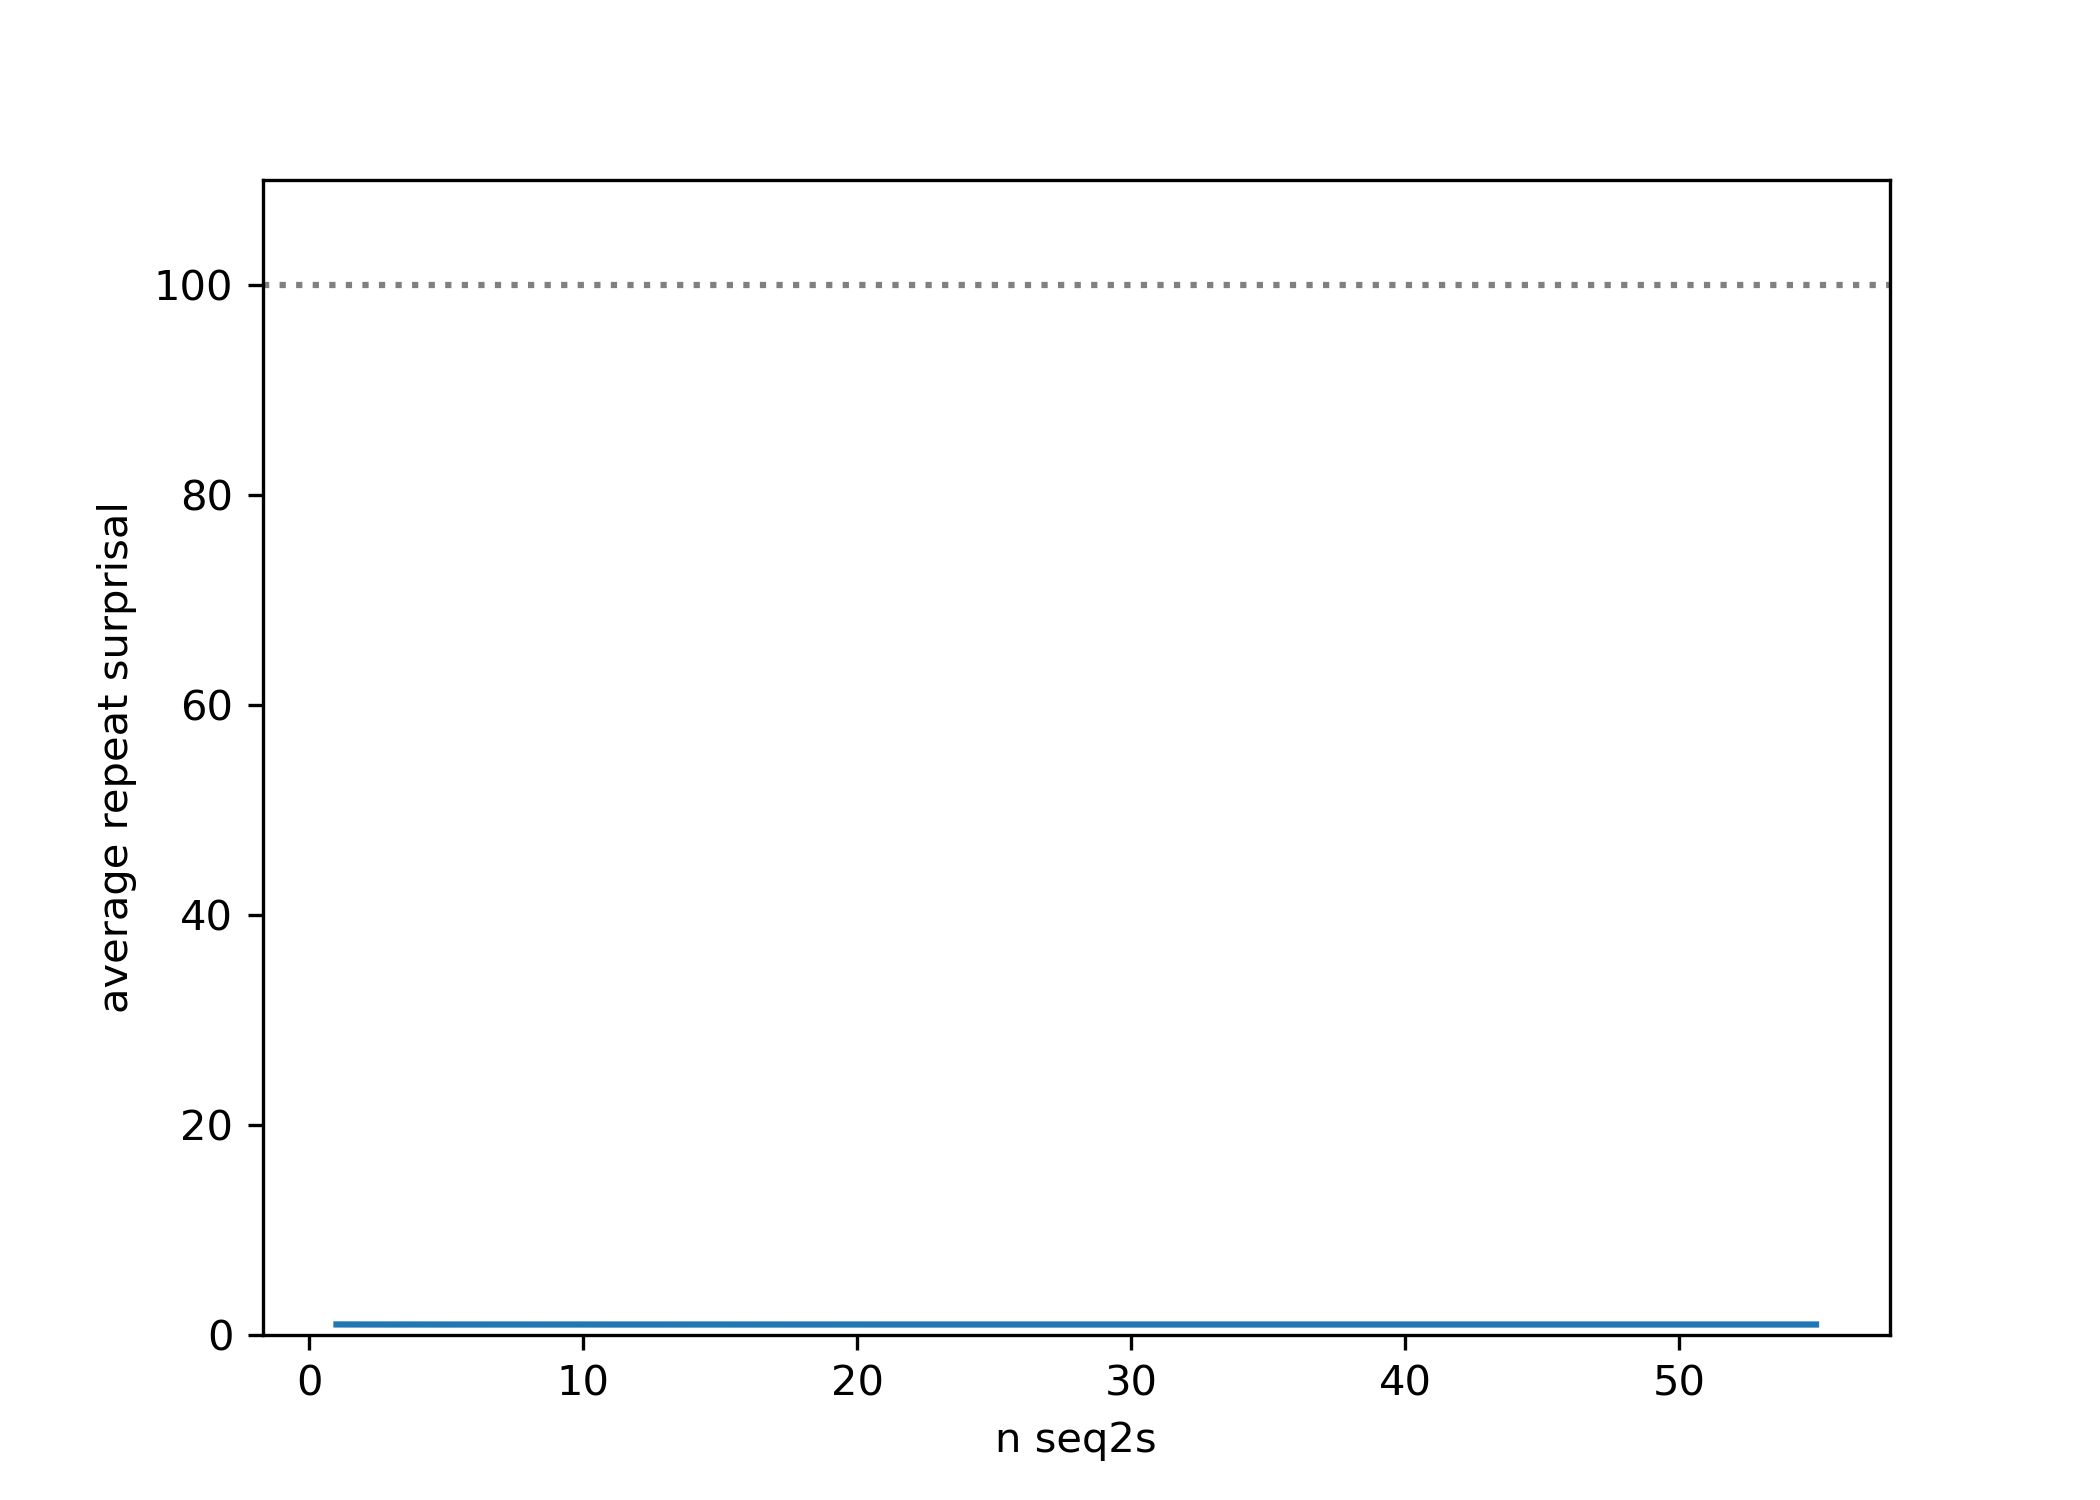
\includegraphics[width=.4\textwidth]{appendix/repeat_surprisal_nseq2.png}}\quad
  \subfloat[same as (c), but scaled y-axis (repeat surprisal) range to 0.9925  - 1.0125 percent]{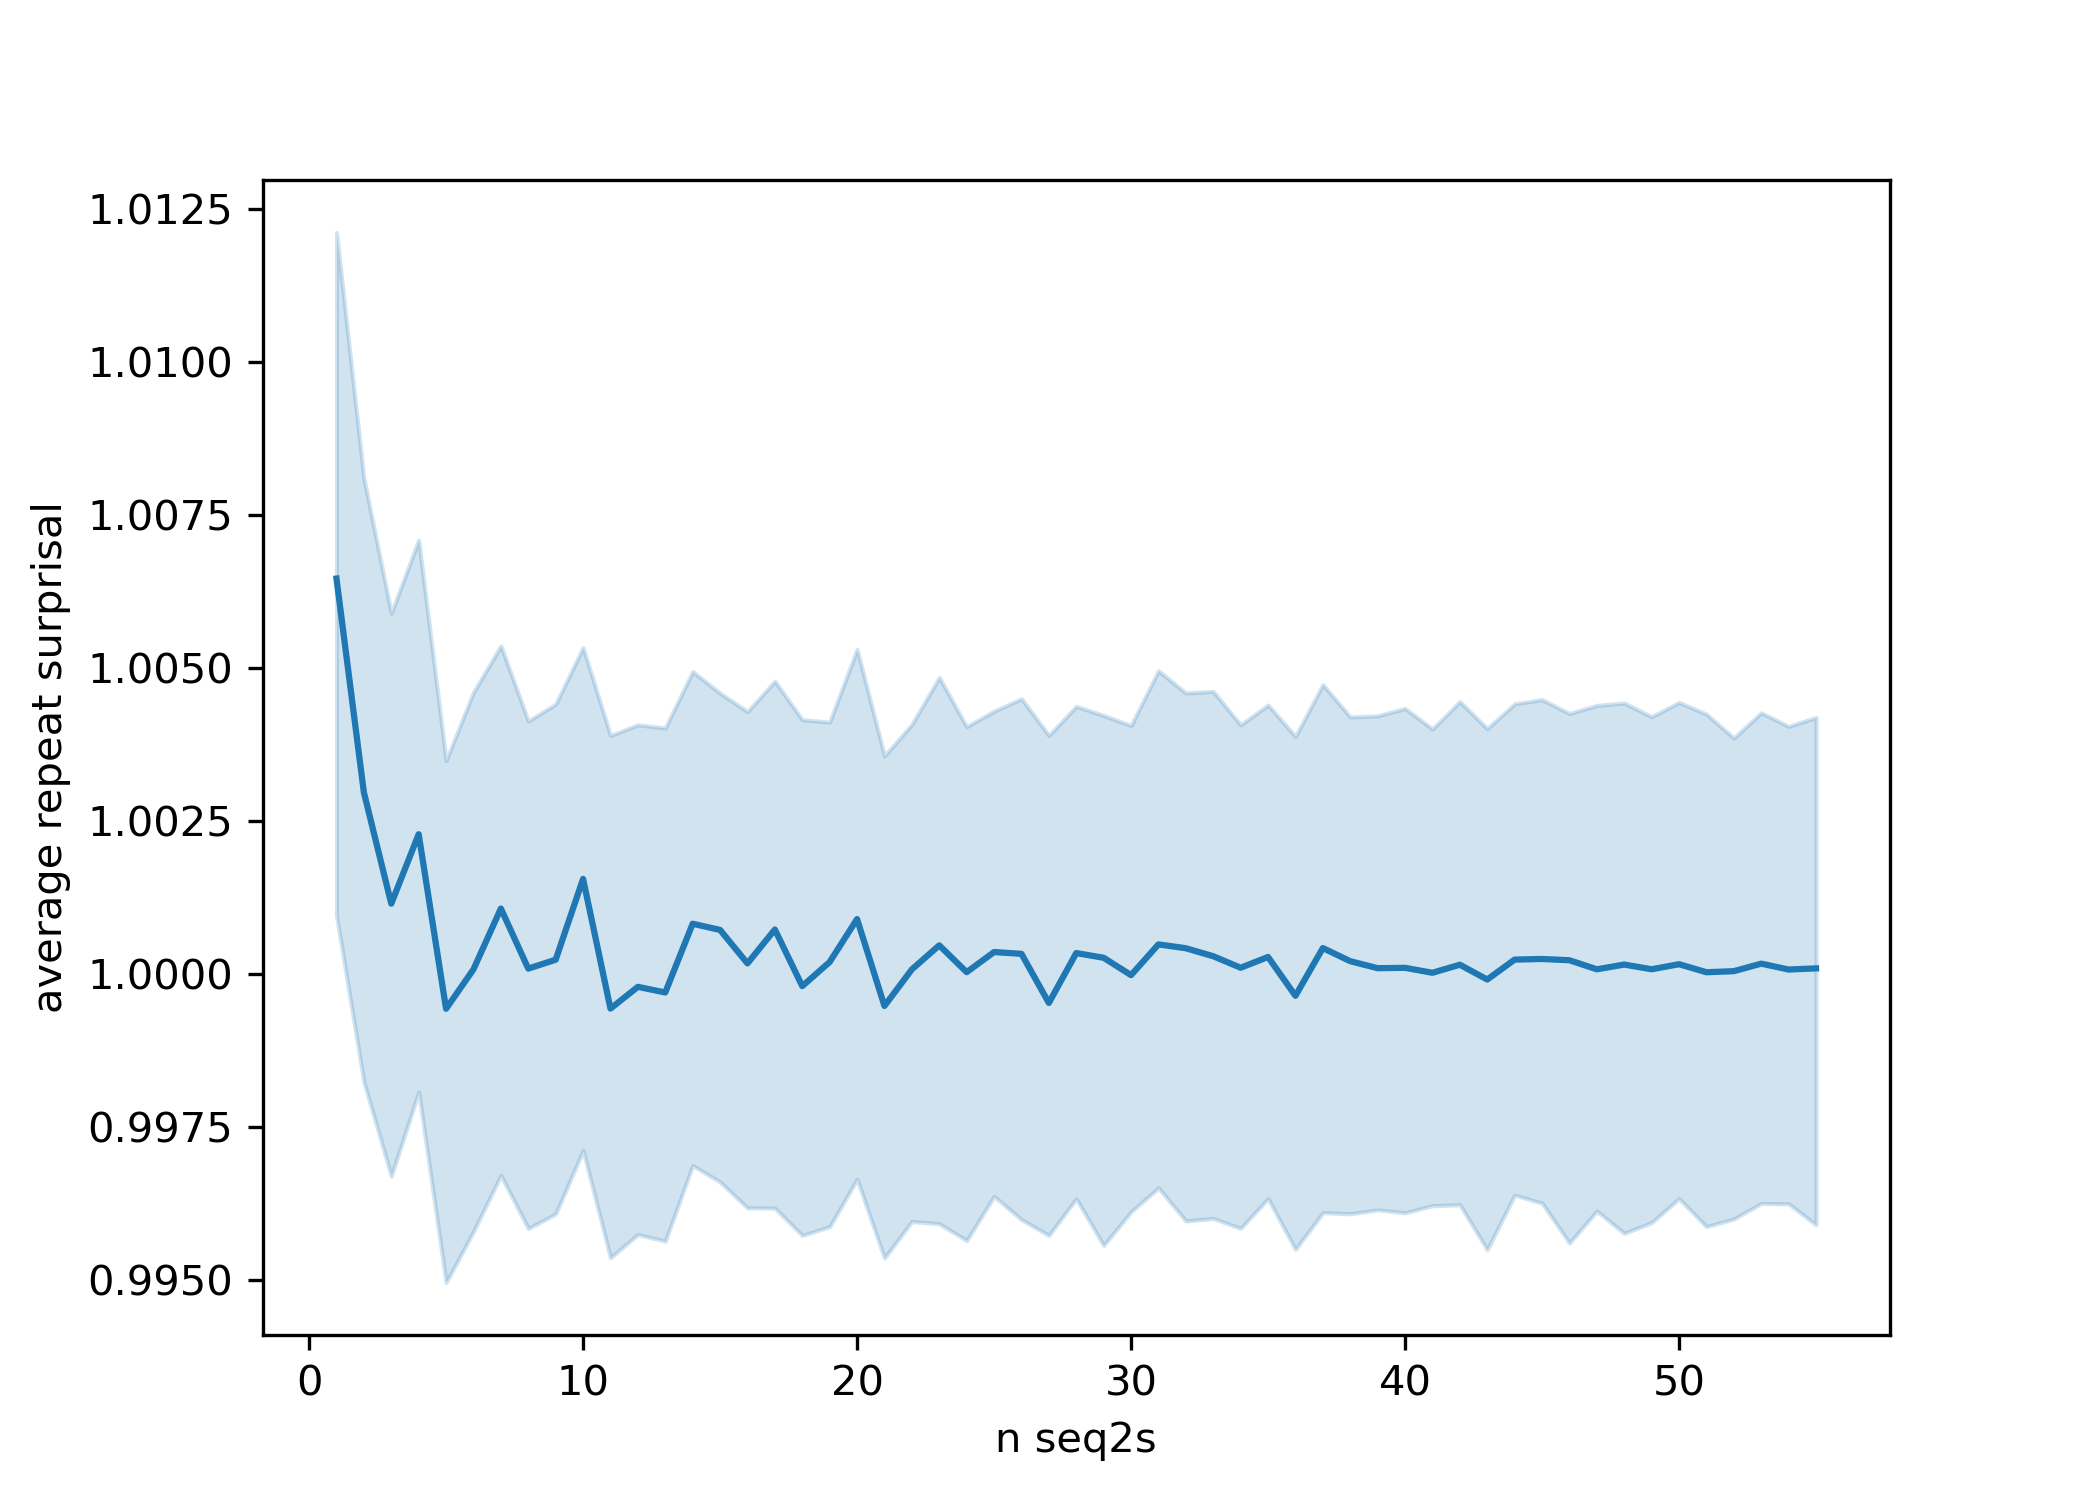
\includegraphics[width=.4\textwidth]{appendix/repeat_surprisal_nseq2_closeup.png}}
  \caption{Average surprisal of the median of control-sentences dependent on the amount of control-sentences used (a,b). Average repeat surprisal dependent on the amount of control-sequences used (c,d). Experiments were repeated 50 times.}
  \label{fig:rs_10_controls}
\end{figure}


\subsection{Sampling of Synonyms}\label{app:syn_sampling}

In order to create the SYN condition of \ref{exp:word_swap}, synonyms for the nouns verbs of our sentences are needed.

For sampling we created a synonym candidate list with help of \url{https://www.thesaurus.com/}, \parencite{miller_wordnet_1995} and \href{http://paraphrase.org}{PPDB} \parencite{pavlick_ppdb_2015} (accessed with code from \href{https://github.com/makcedward/nlpaug}{nlpaug}).
This synonym candidate list was proofread by at one (nonce-sentences) or two (wikitext sentences) native English speakers. The entire list of synonyms can be found \href{https://docs.google.com/spreadsheets/d/1H95LVB7VJXTtizHpGqHZp7Ky9NsPlMgj-W6yAFc6LOI/edit}{here}.

\begin{table} \centering
    \begin{threeparttable}
        \begin{tabular}{ p{0.39\linewidth} | c | c c c}
            \hline
            \thead{Sentence} & \thead{Target word} & \multicolumn{3}{c}{\thead{Synonyms}} \\
            \hline\hline
            the section on current routes adds nothing to the info . & section & part	& passage & paragraph \\
            \hline
            the section on current routes adds nothing to the info . & adds & appends	& supplements & \\
        \end{tabular}
        \caption{Example synonyms} \label{Tab:syn_sampling}
    \end{threeparttable}
\end{table}

We actively decided against generating these synonyms with LMs to avoid a circular argument:
In the hypothetical case in which synonyms are sampled with a LM we test our transformers on that LMs semantic knowledge of contextual synonyms, and not the human semantic knowledge of synonyms.
For instance, the generated synonyms may only are synonyms which are easily learned by LMs because of certain word distributions.
The tested transformers may as well easily pick up on these synonyms.
Subsequently, the tested transformers may have an easier time predicting these synonyms during our experiment, whilst there may exist another class of synonyms which does not show such a property.
We thus would arrive at the wrong conclusion.


\subsection{Word-swap Experiment detailed Setup}\label{app:word_swap_setup}

\begin{itemize}
    \item[RPT] All 60 sentences (sec. \ref{met:sentences_used}) are used to create 60 test sequences. For each test sequence, one sentence is used as encoding- and test-sentence (such that encoding- and test-sentence are the same).
    \item[SYN] For each of the 60 sentences synonyms were sampled for both the marked verb and noun. The 60 original sentences are used as encoding-sentence. They are paired with a test-sentence which is the same except for the word at the marked position: instead of the original word, a semantically fitting synonym is inserted.
    \item[ARB] As in SYN, the 60 original sentences are used as encoding-sentences. They are paired with a test-sentence in which the marked word is replaced with an arbitrary word within the same part-of-speech category as the original word. The arbitrary nouns and verbs sampled from a list of 200 verbs and 300 nouns respectively. These lists are taken from the nonce-dataset \cite{linzen_assessing_2016}. For each original sentence, $10$ verbs and $10$ nouns are sampled, for a total of $60 \dot 10$ measures.
\end{itemize}
In each condition 10 pairwise-different control-sentences are sampled from the then remaining original $59$ sentences to construct the control sequences.


\subsection{Repeat Experiment: Generalization across transformers}

\begin{figure}[H]
    \centering
    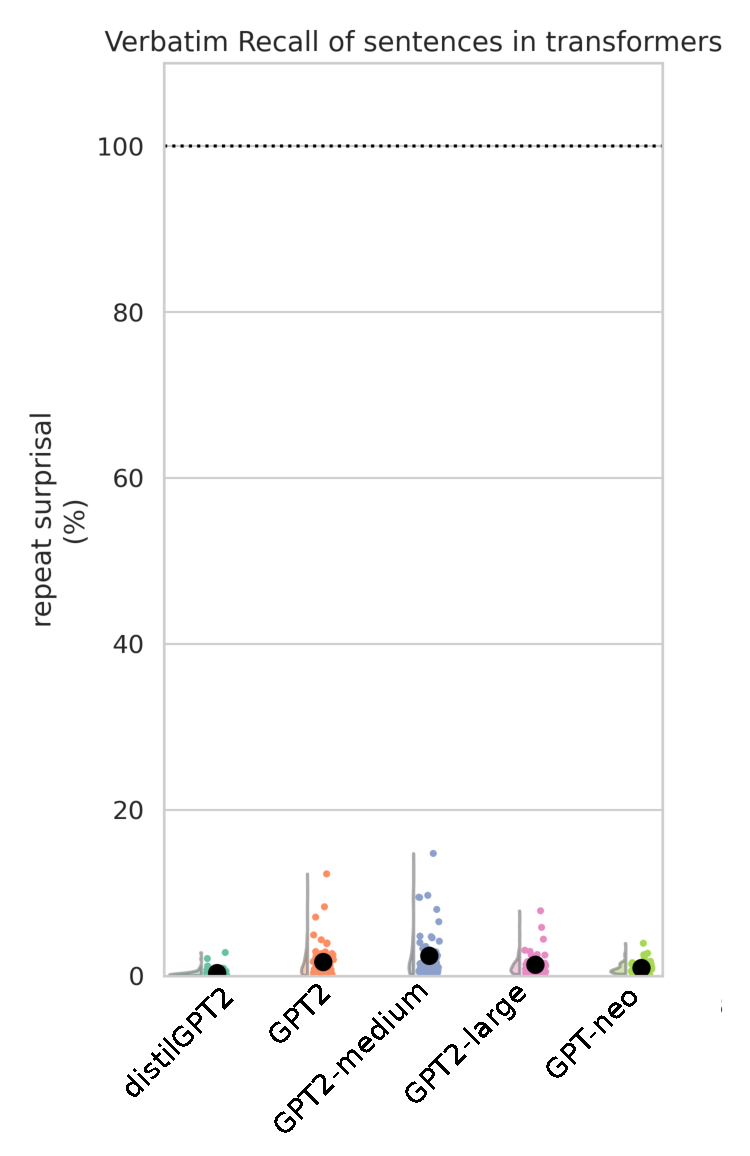
\includegraphics[width=0.5\textwidth]{experiments/repeat_surprisal_all.pdf}
    \caption{Repeat surprisal for different transformer models for verbatim repetition of sentences ($N = 60$). The Y axis shows the repeat surprisal as percentage. The ``raincloud plot'' \parencite{allen_raincloud_2019} shows the distribution of repeat surprisal as kernel density estimate (left). The points (right) are the actual repeat surprisal values for each measure. The black point (right) indicates the mean. Bootstrap $95\%$ confidence intervals are plotted around the mean, but are not visible due the consistency of the repeat surprisal in this experiment.}
    \label{fig:repeat_all}
\end{figure}


\subsection{Repeat Experiment: How M0, M1, M2 and M3 can account for results} \label{app:repeat_null_explanation}

\textbf{M0} fWM, together with the transformers ability to create syntactically coherent sentences suffice to explain the result: every word in the test-sentence is in prior context, and has its probability significantly increased by the M0 fWM. The model now selects the right words based on the syntactic plausibility at each position.
\textbf{M1} fWM heightens the probability of the continuation of the longest to current context matching sequence in the past context.
This results in an increase of probability for exactly the repeated word.
\textbf{M2} fWM operates as M1 fWM, additionally increasing probabilities of words within the same POS-category as the continued word.
Since probabilities for the continued word itself are still increased, the low repeat surprisal is conceivable.
\textbf{M3} fWM works analogous to M2 fWM just increasing probabilities for synonyms of the continued word instead of within-POS-category words.


\subsection{Word-swap experiment: Generalization across transformers}

\begin{figure}[H]
    \centering
    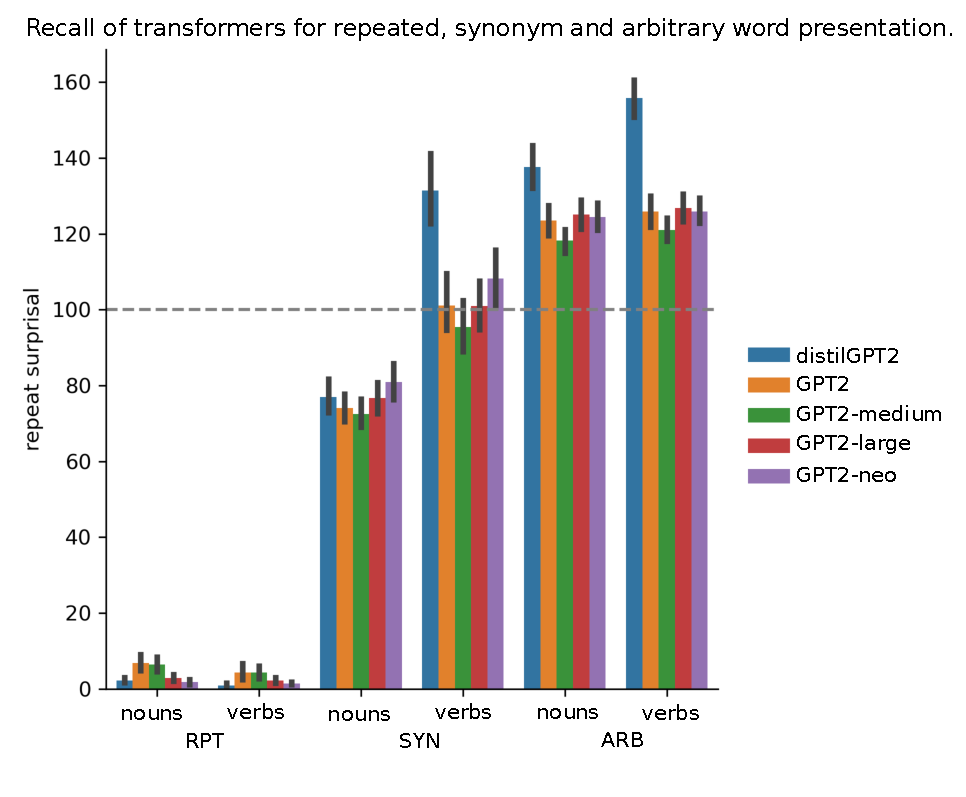
\includegraphics[width=\textwidth]{experiments/word_swap_all.pdf}
    \caption{Bar plot of repeat surprisal for the RPT, SYN and ARB conditions in the word swap experiment across transformers. The bars indicates the mean, the whiskers denote the $95\%$ confidence interval. In most conditions the transformers perform very similar to each other.}
    \label{fig:word_swap_all}
\end{figure}


\end{document}
